% Chapter Template

% Main chapter title
%\chapter[toc version]{doc version}
\chapter{Multi-source domain adaptation}

% Short version of the title for the header
%\chaptermark{version for header}

% Chapter Label
% For referencing this chapter elsewhere, use \ref{ChapterTemplate}
\label{chp:domain_adaptation}

% Write text in here
% Use \subsection and \subsubsection to organize text

\begin{tcolorbox}
    \small{
    Some parts of this chapter were originally published in or adapted from:
    \begin{itemize}
        \item[] \cite{ThesisFrancisco} \bibentry{ThesisFrancisco} (presented in \Secref{sec:da_sensors})
        \item[] \cite{MODAFM} \bibentry{MODAFM} (presented in \Secref{sec:modafm})
    \end{itemize}

    The Master's thesis \cite{ThesisFrancisco} was supervised by Jaime S. Cardoso and co-supervised by Diogo Pernes.
    }
\end{tcolorbox}

\section{Introduction}
\label{sec:chp3_intro}
In Chapter \ref{chp:networked_data_streams}, we have addressed the situation where the set of entities was the same at training and testing time. The goal there was to exploit inter-correlations between entities to learn better generative models for each individual entity. Now, we focus on the problem of learning a discriminative model for one particular entity (the \newterm{target}) for which no annotated data is available. Assuming some invariance properties, we can hope to accomplish this task by learning a discriminative model using the combination of annotated data from the remaining entities (the \newterm{sources}) and unlabeled data from the target entity. Since entities do not need to (and generally do not) correspond to physical objects and may refer to different contexts where the data was collected, they are more commonly called \newterm{domains} and the problem itself is known as \newterm{domain adaptation} (DA). In the following, we motivate the practical importance of this problem and summarize our contributions.

Supervised training of deep neural networks has achieved outstanding results on multiple learning tasks greatly due to the availability of large and rich annotated datasets. Unfortunately, annotating such large-scale datasets is often prohibitively time-consuming and expensive. Furthermore, in many practical cases, it is not possible to collect annotated data with the same characteristics as the test data, and, as a result, training and test data are drawn from distinct underlying distributions. As a consequence, the model performance tends to decrease significantly on the test data. The goal of DA algorithms is to minimize this gap by finding transferable knowledge from the source to the target domain. Sometimes, it is assumed that a small portion of labeled target data are available at training time -- a setting that is known as \newterm{semi-supervised} DA (e.g.\ \citet{Daume2010, Donahue2013, Kumar2010, Saito2019, Yao2015}). In this chapter, we focus mostly on the more challenging scenario, where no labeled target data are available for training -- known as \newterm{unsupervised} DA (e.g.\ \citet{Baktashmotlagh2013, Ganin2015, Kang2019, Long2016a, Zhao2018}). The DA problem, in its semi-supervised and unsupervised variants, has received increased attention in recent years, both from theoretical (e.g.\ \citet{BenDavid2010, BenDavid2007, Blitzer2008, Cortes2014, Gopalan2013, Hoffman2018, Zhao2019}) and algorithmic perspectives (e.g.\ \citet{Ajakan2014, Becker2013, Fernando2013, Jhuo2012, Long2015, Louizos2015, Sun2016, Tzeng2017}). In many situations, the annotated training data may consist of a combination of distinct datasets, some of which may be closer or farther away from the target data. Finding nontrivial ways of combining multiple datasets to approximate the target distribution and extracting relevant knowledge from such combination is the purpose of multi-source DA algorithms (e.g.\ \citet{Kim2017, Guo2018, Hoffman2018, Mansour2009, Sebag2019, Zhang2015, Zhao2018}) and is also our main focus in this chapter.

The remainder of the chapter is organized as follows: i) we formalize the problem and provide some useful background by reviewing some important theoretical results and state of the art algorithms (\Secref{sec:chp3_background}); ii) we discuss some exploratory solutions for this problem in the context of sensor networks (\Secref{sec:da_sensors}); and finally iii) we present our own novel algorithm for unsupervised multi-source domain adaptation (\Secref{sec:modafm}).

\section{Background}
\label{sec:chp3_background}
We start by analyzing the problem of DA from a theoretical perspective and then we overview the main approaches that constitute the state of the art. Although some authors have considered the problem of DA for regression problems (e.g.\ \citet{Cortes2011}, \citet{Zhao2018}), the literature on classification is far more vast. Moreover, many of the results and methods explained in this section can be extended to regression problems with minor modifications. For these reasons, we shall focus our discussion mostly on classification.

\subsection{Theoretical foundation}
\label{sec:da_theory}

\subsubsection{Single source setting}
\label{sec:da_theory_ss}
\citet{BenDavid2010} developed a rigorous yet comprehensive theoretical model for domain adaptation that we summarize here. This formulation enlightens the intrinsic difficulties associated with this task and provides a deep foundation to many of the algorithms we discuss in this chapter and, particularly, to our own approach, presented in \Secref{sec:modafm}.

Before we present and discuss the most important results, let us introduce a few preliminary definitions. A \newterm{domain} $\gD$ is defined by a joint distribution $p_\gD(\rvx, \rvy)$ over input features $\rvx \in \gX$ and target variables $\rvy \in \gY$, where $\gX$ and $\gY$ denote the input and target spaces, respectively. For the domain adaptation task to be well defined, at least two domains must be considered: a \newterm{source} domain $\gS$, with joint distribution denoted by $p_\gS(\rvx, \rvy)$, from which abundant annotated data is usually available, and a \newterm{target} domain $\gT$, with joint distribution $p_\gT(\rvx, \rvy)$, from which scarce or even zero annotated data is available at training time. Following most classical results from statistical learning theory, \citet{BenDavid2010} focused on binary classification, thus $\gY = \{0, 1\}$. Under this setting, it is possible to define a \newterm{labeling function} $f_\gD: \gX \mapsto [0, 1]$ for each domain, given by $f_\gD(\vx) = p_\gD(\ry=1 \mid \vx)$. A \newterm{hypothesis} is any function $h: \gX \mapsto \{0,1\}$ and a set $\gH$ of these functions is called a \newterm{hypothesis class}. The expected absolute difference between $h$ and $f_\gD$ is called the \newterm{risk} (or \newterm{error}) of hypothesis $h$ (with respect to the labeling function $f_\gD$):
\begin{equation}
    \label{eq:risk}
    \epsilon(h,f_\gD) \triangleq \E_{\rvx \sim p_\gD} \left[|h(\rvx) - f_\gD(\rvx)|\right].
\end{equation}
We use $\epsilon_\gS(h)$ and $\epsilon_\gT(h)$ as shorthands for $\epsilon(h,f_\gS)$ and $\epsilon(h,f_\gT)$ and refer to them as the source and target risks (or errors), respectively. The empirical estimates of these are denoted as $\widehat{\epsilon}_\gS(h)$ and $\widehat{\epsilon}_\gT(h)$, respectively.

Given two domains $\gD$ and $\gD'$ and a hypothesis class $\gH$, the $\gH$-divergence provides a distance measure between the marginal distributions of features in $\gD$ and $\gD'$ (according to $\gH$):
\begin{equation*}
    \label{eq:h_div}
    d_{\gH}(\gD,\gD') \triangleq \sup_{h \in \gH} 2 |\mathrm{Pr}_{\gD}(\1_h) - \mathrm{Pr}_{\gD'}(\1_h)|,
\end{equation*}
where $\1_h \triangleq \{\vx \in \gX: h(\vx)=1\}$ and $\mathrm{Pr}_{\gD}(\1_h)$ is the probability assigned by the density $p_\gD(\rvx)$ to the subset $\1_h \subseteq \gX$. As is often the case, when the true underlying marginal distributions are unknown or intractable but finite sets of (unlabeled) samples from both domains are available, an empirical $\gH$-divergence can be constructed by replacing the true probabilities $\mathrm{Pr}_{\gD}(\1_h)$ and $\mathrm{Pr}_{\gD'}(\1_h)$ by the respective empirical estimates. Remarkably, under weak conditions on the hypothesis class, computing this empirical $\gH$-divergence is equivalent to finding the hypothesis in $\gH$ that maximally discriminates between samples of the two domains. This result is enunciated formally in Lemma \ref{lemma:emp_h_div} and, as we shall see later, is exploited by adversarial-based approaches for domain adaptation.
\begin{lemma}
    \label{lemma:emp_h_div}
    (Lemma 2 from \citet{BenDavid2010}) Let $\gH$ be a hypothesis class such that if $h \in \gH$ then $1-h \in \gH$. Given two sets $\widehat{\gD}$ and $\widehat{\gD}'$ of $n$ samples each drawn from two domains $D$ and $D'$, the empirical $\gH$-divergence between $\gD$ and $\gD'$ is given by:
    \begin{equation}
        \widehat{d}_{\gH}(\gD,\gD') = 2 \left(1 - \min_{h \in \gH} \left[\frac{1}{n} \sum_{\vx:~h(\vx)=1} \1_{\vx \in \widehat{\gD}} + \frac{1}{n} \sum_{\vx:~h(\vx)=0} \1_{\vx \in \widehat{\gD}'}\right]\right).
    \end{equation}
\end{lemma}
Note that if the two sets $\widehat{\gD}$ and $\widehat{\gD}'$ can be discriminated perfectly by a hypothesis $h \in \gH$ (i.e.\ if there is an $h \in \gH$ such that $h(\vx) = 0$ if $x \in \widehat{\gD}$ and $h(\vx) = 1$ if $x \in \widehat{\gD}'$), then $\widehat{d}_{\gH}(\gD,\gD')$ is maximum and equal to 2.

For any hypothesis class $\gH$, we may define the \newterm{symmetric difference hypothesis class} $\gH \Delta \gH$ as:
\begin{equation}
    \label{eq:h_delta_h}
    \gH \Delta \gH \triangleq \{l: l(\vx) = h(\vx) \oplus h'(\vx), \; h, h' \in \gH\},
\end{equation}
where $\oplus$ denotes the ``exclusive or" (xor) operation. Combining this definition with \eqref{eq:h_div}, the definition of $\gH \Delta \gH$-divergence, which happens to play a major role in Theorem \ref{thm:da_bound_single_source}, follows immediately. This theorem is the main result in this section as it provides an upper bound for the target risk given the source risk and the $\gH \Delta \gH$-divergence between the source and target domains.
\begin{theorem}
    \label{thm:da_bound_single_source} (Theorem 2 from \citet{BenDavid2010}) Let $\gH$ be a hypothesis class with VC-dimension $d$. Consider $n$ unlabeled samples drawn from each of the two domains $\gS$ (source) and $\gT$ (target). Then, for every $h \in \gH$ and any $\delta \in (0,1)$, with probability at least $1-\delta$ over the choice of samples,
    \begin{equation}
        \label{eq:da_bound_single_source}
        \epsilon_\gT(h) \leq \epsilon_\gS(h) + \frac{1}{2} \widehat{d}_{\gH \Delta \gH}(\gS, \gT) + \lambda + 2\sqrt{\frac{2d\log(2n) + \log(\frac{2}{\delta})}{n}},
    \end{equation}
    where $\lambda \triangleq \min_{h \in \gH} \epsilon_\gS(h) + \epsilon_\gT(h)$.
\end{theorem}
This bound immediately confirms the intuition that a low target error can be achieved by training a classifier to minimize the error in the source domain, provided that the marginal distributions of features are similar (i.e.\ $\widehat{d}_{\gH \Delta \gH}(\gS, \gT)$ is small) and a low error on the combination of the two domains can be achieved (i.e.\ $\lambda$ is also small). A deeper and more complete interpretation of this bound shall be provided later on, when we take into account the fact that, by applying deep neural networks, we can not only construct rich hypothesis classes but also manipulate and learn feature representations. The latter observation suggests that this kind of classifiers may also have an impact on the $\widehat{d}_{\gH \Delta \gH}(\gS, \gT)$ and $\lambda$ terms in \eqref{eq:da_bound_single_source}, which will indeed be the case.

\subsubsection{Multi-source setting}
\label{sec:da_theory_ms}
So far we have only considered the setting where a single source domain was available. However, in many practical cases, the annotated training dataset consists of a collection of subdatasets, each one belonging to its own domain. Therefore, it makes sense to consider $k$ distinct source domains $\gS_1, \gS_2, \dots, \gS_k$ and, in particular, to see how Theorem \ref{thm:da_bound_single_source} can be generalized to this setting.
\begin{theorem}
    \label{thm:da_bound_multi_source}
    (Theorem 2 from \citet{Zhao2018}) Let $\gH$ be a hypothesis class with VC-dimension $d$. Consider $n$ unlabeled samples drawn from the target domain $\gT$ and $n/k$ annotated samples drawn from each of the $k$ source domains $\gS_1, \gS_2, \dots, \gS_k$. Then, for every $h \in \gH$, any $\valpha \in [0,1]^k: \sum_{j=1}^k \evalpha_i = 1$, and any $\delta \in (0,1)$, with probability at least $1-\delta$ over the choice of samples,
    \begin{equation}
        \label{eq:da_bound_multi_source}
        \epsilon_\gT(h) \leq \sum_{j=1}^k \evalpha_j \left(\widehat{\epsilon}_{\gS_j}(h) + \frac{1}{2} \widehat{d}_{\gH \Delta \gH}(\gS_j, \gT)\right) + \lambda_\valpha + O \left(\sqrt{\frac{1}{n} \left(\log \frac{1}{\delta} +d \log \frac{n}{d} \right)} \right),
    \end{equation}
    where $\lambda_\valpha \triangleq \min_{h \in \gH} \epsilon_\gT(h) + \sum_{j=1}^k \evalpha_j \epsilon_{\gS_j}(h)$.
\end{theorem}
Unsurprisingly, the bound in Theorem \ref{thm:da_bound_multi_source} is essentially a convex combination of the bounds provided by Theorem \ref{thm:da_bound_single_source} for each individual source domain. Thus, the same interpretation applies here. Nonetheless, the source weights $\valpha$ provide an extra degree of freedom that should be taken into account. Depending on how much each source domain differs from the target, it may be beneficial to weight each source domain differently. Adjusting these weights is therefore an extra non-trivial task, exclusive to the multi-source setting, that may have a significant impact in the performance of the domain adaptation algorithm.

\subsection{State of the art}
\label{sec:da_sota}
We now do a brief overview of the most relevant DA algorithms, both in the single source and multi-source settings.

As we have just seen from a theoretical point of view, the success of the DA task depends on how similar the target domain is to the source(s), which is equivalent to saying that some properties of the underlying distributions must be invariant across domains. Different DA algorithms can therefore be categorized according to the invariance properties they assume.

\subsubsection{Target shift}
\label{sec:target_shift_sota}
\begin{figure}
    \centering
    \begin{tikzpicture}[every loop/.style={},thick,
        main node/.style={circle,draw},font=\sffamily\Large\bfseries]

        \node[main node,minimum size=1.5cm] (D) {$\gD$};
        \node[main node,minimum size=1.5cm] (y) [right=1.5cm of D] {$\ry$};
        \node[main node,minimum size=1.5cm] (x) [right=1.5cm of y] {$\rvx$};

        \draw[->]
        (D) edge (y)
        (y) edge (x);

    \end{tikzpicture}
    \caption{Graphical representation of the target shift setting as a Bayesian network.}
    \label{fig:target_shift}
\end{figure}
In the \newterm{target shift} setting, only the marginal distribution of labels is allowed to vary across domains. A practical example where this assumption may be realistic is when the label $\ry$ represents having or not a certain disease and the input features $\rvx$ are symptoms. It is plausible to assume that the prevalence of the disease may vary over time or across different populations, but the probability of some symptom being present or absent given that one has or not the disease should remain constant. Thus, as implied by \Figref{fig:target_shift}, the joint distribution of any domain $\gD$ is assumed to factorize as $p_\gD(\rvx, \ry) = p(\rvx \mid \ry) p_\gD(\ry)$, where $p(\rvx \mid \ry)$ is domain-invariant. By further assuming that $\mathrm{Supp}(p_\gT(\ry)) \subseteq \mathrm{Supp}(p_\gS(\ry))$, we have:
\begin{align}
    p_\gT(\ry \mid \rvx) &\propto p(\rvx \mid \ry) p_\gT(\ry) \nonumber\\
    &= p(\rvx \mid \ry) p_\gS(\ry) \frac{p_\gT(\ry)}{p_\gS(\ry)} \nonumber\\
    &\propto p_\gS(\ry \mid \rvx) \frac{p_\gT(\ry)}{p_\gS(\ry)}.
\end{align}
Thus, if the class ratios $p_\gT(\ry)/p_\gS(\ry)$ are known, the problem of DA under target shift is solved by learning a probabilistic classifier on the source domain, reweighting it with the class ratios, and then normalizing the class scores. Therefore, the literature for DA under target shift focuses on estimating class ratios when these are unknown and cannot be estimated directly from the training data, due to the absence of labels for the target samples.

An elegant and simple solution to this problem was proposed by \citet{Lipton2018}. Specifically, for any classifier $h: \gX \mapsto \gY$ trained with labeled data from the source domain, the target shift assumption implies that $p_{\gT}(h(\rvx) \mid \ry) = p_{\gS}(h(\rvx) \mid \ry)$ and hence:
\begin{align}
    p_{\gT}(h(\rvx)) &= \sum_{\ry} p_{\gT}(h(\rvx) \mid \ry) p_{\gT}(\ry) \nonumber\\
    \allowdisplaybreaks
    &= \sum_{\ry} p_{\gS}(h(\rvx) \mid \ry) p_{\gT}(\ry) \label{eq:estim_class_dist}\\
    \allowdisplaybreaks
    &= \sum_{\ry} p_{\gS}(h(\rvx), \ry) \frac{p_{\gT}(\ry)}{p_{\gS}(\ry)}. \label{eq:estim_class_ratio}
\end{align}
Note that $p_{\gS}(h(\rvx) \mid \ry)$, $p_{\gS}(h(\rvx), \ry)$, and $p_{\gS}(\ry)$ can all be estimated from labeled source samples and $p_{\gT}(h(\rvx))$ can be estimated from unlabeled target samples. Thus, one can either use \eqref{eq:estim_class_dist} to estimate $p_{\gT}(\ry)$ or \eqref{eq:estim_class_ratio} to estimate class ratios directly.

Other approaches involve learning class-dependent weights to match the mean conditional features of source data with the mean marginal features of target data in a reproducing kernel Hilbert space (e.g.\  \citet{Iyer2004}, \citet{Zhang2013}), or require density estimation to model $p(\rvx \mid \ry)$ (e.g.\ \citet{Chan2005}, \citet{Storkey2009}).

\subsubsection{Conditional shift}
\label{sec:cond_shift_sota}
\begin{figure}
    \centering
    \begin{tikzpicture}[every loop/.style={},thick,
        main node/.style={circle,draw},font=\sffamily\Large\bfseries]

        \node[main node,minimum size=1.5cm] (y) {$\ry$};
        \node[main node,minimum size=1.5cm] (x) [right=1.5cm of y] {$\rvx$};
        \node[main node,minimum size=1.5cm] (D) [right=1.5cm of x] {$\gD$};

        \draw[->]
        (y) edge (x)
        (D) edge (x);

    \end{tikzpicture}
    \caption{Graphical representation of the conditional shift setting as a Bayesian network.}
    \label{fig:cond_shift}
\end{figure}
In the \newterm{conditional shift} setting, the marginal distribution of labels is constant and the conditional of features given labels may change across domains. This scenario is represented in \Figref{fig:cond_shift}, from which it becomes clear that the joint distribution takes the form $p_{\gD}(\rvx, \ry) = p(\ry) p_{\gD}(\rvx \mid \ry)$, where $p(\ry)$ is domain-invariant. Besides being less realistic than other assumptions, DA under conditional shift is in general an ill-posed problem. Nonetheless, \citet{Zhang2013} show that identifiability of $p_{\gT}(\rvx \mid \ry)$ holds when it is assumed that, for any given $y$, $p_{\gT}(\rvx \mid y)$ only differs from $p_{\gS}(\rvx \mid y)$ in location and scale and derive a kernel-based approach to estimate these parameters.

\subsubsection{Concept shift}
\label{sec:concept_shift_sota}
\begin{figure}
    \centering
    \begin{tikzpicture}[every loop/.style={},thick,
        main node/.style={circle,draw},font=\sffamily\Large\bfseries]

        \node[main node,minimum size=1.5cm] (x) {$\rvx$};
        \node[main node,minimum size=1.5cm] (y) [right=1.5cm of x] {$\ry$};
        \node[main node,minimum size=1.5cm] (D) [right=1.5cm of y] {$\gD$};

        \draw[->]
        (x) edge (y)
        (D) edge (y);

    \end{tikzpicture}
    \caption{Graphical representation of the concept shift setting as a Bayesian network.}
    \label{fig:concept_shift}
\end{figure}
\newterm{Concept shift} refers to the situation where the marginal feature distributions $p(\rvx)$ are constant but the conditional distribution of the target variable $p_{\gD}(\ry \mid \rvx)$ is domain-dependent, thus $p_{\gD}(\rvx, \ry) = p(\rvx)p_{\gD}(\ry \mid \rvx)$, as implied by \Figref{fig:concept_shift}. When the change happens over time, this setting is also known as \newterm{concept drift} (\citet{Webb2018}). The literature on concept drift is vast and focuses mostly on the detection of its occurrence so that the model can be updated using new data. \citet{Gama2014} overview the most popular techniques to address this problem.

\subsubsection{Covariate shift}
\label{sec:cov_shift_sota}
\begin{figure}
    \centering
    \begin{tikzpicture}[every loop/.style={},thick,
        main node/.style={circle,draw},font=\sffamily\Large\bfseries]

        \node[main node,minimum size=1.5cm] (D) {$\gD$};
        \node[main node,minimum size=1.5cm] (x) [right=1.5cm of D] {$\rvx$};
        \node[main node,minimum size=1.5cm] (y) [right=1.5cm of x] {$\ry$};

        \draw[->]
        (D) edge (x)
        (x) edge (y);

    \end{tikzpicture}
    \caption{Graphical representation of the covariate shift setting as a Bayesian network.}
    \label{fig:cov_shift}
\end{figure}
\newterm{Covariate shift} is by far the most common assumption and therefore the most widely addressed setting in the DA literature. As implied by the graphical representation in \Figref{fig:cov_shift}, here the conditional distribution of labels given features is constant and the marginal distribution of features is domain-dependent. Thus, $p_\gD(\rvx, \ry) = p(\ry \mid \rvx) p_\gD(\rvx)$, where $p(\ry \mid \rvx)$ is constant across domains. This assumption might hold for instance in image classification problems where the domain shift is caused by different sensors or lighting conditions.

Since $p_\gT(\ry \mid \rvx) = p_\gS(\ry \mid \rvx)$, infinite labeled data from the source domain and a consistent estimator of this conditional distribution would solve this DA task. However, the former is obviously unrealistic and therefore the problem should be analyzed taking into account that the available data is finite. Let $\ell(\cdot, \cdot)$ be any loss function for the supervised learning problem. The goal is then to find an unbiased estimator of the target loss $\E_{\rvx, \ry \sim p_\gT} \left[\ell(h(\rvx),\ry)\right]$ when no labeled samples from the target domain are available. Following \citet{Sugiyama2007}, if the marginal densities $p_\gS(\rvx)$ and $p_\gT(\rvx)$ are known and assuming $\mathrm{Supp}(p_\gT(\rvx)) \subseteq \mathrm{Supp}(p_\gS(\rvx))$, this estimator can be obtained using \newterm{importance weights} $w(\rvx) \triangleq p_\gT(\rvx)/p_\gS(\rvx)$:
\begin{align}
    \E_{\rvx, \ry \sim p_\gT} \left[\ell(h(\rvx),\ry)\right] &= \sum_{\ry} \int l(h(\rvx),\ry) p_\gT(\rvx, \ry) \d\rvx \nonumber\\
    &= \sum_{\ry} \int \ell(h(\rvx),\ry) p(\ry \mid \rvx) p_\gT(\rvx) \d\rvx \nonumber\\
    &= \sum_{\ry} \int \frac{p_\gT(\rvx)}{p_\gS(\rvx)} \ell(h(\rvx),\ry)  p(\ry \mid \rvx) p_\gS(\rvx) \d\rvx \nonumber\\
    &= \sum_{\ry} \int w(\rvx) \ell(h(\rvx),\ry)  p_\gS(\rvx, \ry) \d\rvx \nonumber\\
    &= \E_{\rvx, \ry \sim p_\gS} \left[w(\rvx) \ell(h(\rvx),\ry)\right].
\end{align}
Hence, $(1/n) \sum_{i=1}^{n} w(\vx_i) \ell(h(\vx_i),y_i)$ is an unbiased estimator of the target loss, constructed using only source data, which can therefore be used as the loss for the supervised learning problem. When the marginal distributions are unknown and the feature space is low-dimensional, kernel density estimation techniques can be employed to estimate them (e.g.\ \citet{Shimodaira2000,Sugiyama2007,Cortes2010}). An alternative that removes the constraint on the support of the marginal target distribution is learning a transformation $T: \gX \mapsto \gX$ such that $p_{\gS}(T(\rvx)) = p_{\gT}(\rvx)$, which can be accomplished using optimal transport theory (\citet{Courty2015}). Later approaches aim to relax the covariate shift assumption by trying to align the joint source and target distributions (\citet{Courty2017}) and extend the same principles to the multi-source setting (\citet{Turrisi2020}).

For high-dimensional data (e.g.\ images), where the marginal distributions are typically unknown and hard to estimate from finite data, deep learning models play an important role by providing a successful tool learn semantically rich low-dimensional feature representations. It is then possible to learn a function $g:\gX \mapsto \gZ$ mapping input data to a new feature space $\gZ$ such that $p_{\gT}(g(\rvx))/p_{\gS}(g(\rvx)) \approx 1$, i.e.\ where the marginal feature distributions of the two domains coincide. This approach has the additional benefit of moving the overlapping support assumption to a lower-dimensional space, where it is less likely to be violated than in the original space (e.g.\ pixel space). In this new feature space, the covariate shift has vanished and therefore any classifier $h:\gZ \mapsto \gY$ that achieves low error on the source domain will also perform well in the target. An alternative way of motivating these approaches follows from analyzing again the target risk bound provided in \eqref{eq:da_bound_single_source}. When we presented this bound, we assumed for simplicity that the feature space was fixed and therefore the upper bound would be minimized by minimizing the source risk. However, if the feature space can itself be optimized, the term $\widehat{d}_{\gH \Delta \gH}(\gS, \gT)$ can be minimized by finding a feature space where the source and target marginal distributions coincide. This idea has been exploited extensively in recent years, either by matching the distributions using maximum mean discrepancy (e.g.\ \citet{Long2015,Guo2018}) or, in most cases, using an adversarial neural network (e.g.\ \citet{Zhao2018,Ganin2015,Pei2018,Sebag2019}).

Adversarial-based DA was originally introduced by \citet{Ganin2015} and results from the observation that
computing $\widehat{d}_{\gH \Delta \gH}(\gS, \gT)$ is equivalent to finding a classifier that maximally discriminates between samples of the source and target domains (Lemma \ref{lemma:emp_h_div}). Intuitively, if no classifier exists that can distinguish between source and target features, then the distributions of these two must coincide. Thus, if we have access to sets $\widehat{\gS}$ and $\widehat{\gT}$ of labeled samples from the source domain and unlabeled samples from the target, respectively, we can train a feature extractor network $g:\gX \mapsto \gZ$, a classifier $h:\gZ \mapsto \gY$, and a domain discriminator $d:\gZ \mapsto \{0,1\}$ to solve the following minimax problem\footnote{This objective is merely formal since the 0-1 loss is non-smooth and intractable. In practice, the usual classification losses are used instead.}:
\begin{equation}
    \label{eq:dann_obj}
    \min_{g,h} \max_d \quad \widehat{\epsilon}_\gS(h \circ g) + 1 - \left(\frac{1}{n} \sum_{\vx: d(g(\vx))=1} \1_{\vx \in \widehat{\gS}} + \frac{1}{n} \sum_{\vx: d(g(\vx))=0} \1_{\vx \in \widehat{\gT}}\right),
\end{equation}
where $\circ$ denotes function composition. Several variations to this idea have been proposed so far, aiming to extend it to the multi-source setting (\citet{Zhao2018}), or beyond the covariate shift assumption (\citet{Pei2018}), or both (\citet{Sebag2019}).

\subsubsection{Invariance of causal mechanisms}
\label{sec:causal_da_sota}
The settings we have discussed so far consider all features $\rvx$ as atomic and hence do not take into account how different features interact to produce the target variable $\ry$.  Other approaches drop this limitation by decomposing the feature vector into individual features $\rx_1,\rx_2,\dots,\rx_m$, taking into account the structure of the causal Bayesian network governing the data generating process, and using causal inference tools to identify the target distribution. These methods assume that the flow of cause and effect cannot be reversed by domain shift and therefore changes in distribution are due to different interventions in the same causal graph $\gG$ (e.g.\ presence of additional exogenous variables inducing non-causal associations between features and the target variable). \citet{Bareinboim2016} assume $\gG$ is known and all interventions are perfect (i.e.\ all interventions consist of edge removal operations) and, given some subset $\bar{\rvx} \subset \rvx$, derive conditions for identifiability of $p_\gT(\ry \mid \bar{\rvx})$ given $\gG$ and $p_\gS(\rvx, \ry)$. \citet{Rojas2018} and \citet{Magliacane2018} relax the covariate shift setting by assuming that there exists a strict subset $\bar{\rvx} \subset \rvx$ such that $p_\gD(\ry \mid \bar{\rvx})$ is domain-invariant and propose algorithms to infer $\bar{\rvx}$ given data from multiple source domains.

Despite being (arguably) more trustworthy than purely data-driven approaches, cau-\allowbreak sality-based methods still struggle to be applied in practice. First of all, they depend to some extent on $\gG$ being given. In many applications, domain knowledge is insufficient to build such a graph. Moreover, causal discovery algorithms, which aim to learn the structure of the graph from data, are computationally expensive and, given observational data, can only recover $\gG$ up to its Markov equivalence class, at least when no parametric assumptions are made  (\citet{Peters2014}). Furthermore, these methods are unsuitable to be applied to image data as no meaningful causal reasoning can be built in pixel space and even deep neural networks are still incapable of finding suitable representations for this goal (\citet{Scholkopf2021}).

\section{Adversarial domain adaptation for object counting in videos}
\label{sec:da_sensors}

\subsection{Motivation}
As different sensors are added to and excluded from a network, we should take into account the fact that the sensors used at training time are different from the ones where the model will make predictions. Since domain shifts between different sensors in a network are usually substantial, it is imperative that robust domain adaptation methods are developed that take into account the constraints of the sensor network.

There is a lack of domain adaptation methods focusing on how to handle the temporal component of data. \citet{Chen2019} proposed an algorithm called Temporal Attentive Alignment for implementing DA in video datasets that explicitly attends to temporal dynamics and \citet{Liu2014} proposed a spatio-temporal DA model named TrCbrBoost for classifying land use. It should be noted, though, that both only deal with a single-source-single-target setting, which is simpler than the multi-source case present when dealing with sensor networks.

For dealing with a multi-source setting, adversarial approaches have proven successful. \citet{Zhao2018} introduced an algorithm called multi-source domain adversarial networks (MDAN) that makes use of $k$ domain discriminators that aim to distinguish between the target and the $k$ source domains. MDAN showed superior performance when compared to other state of the art methods on the task of counting vehicles in images obtained from city cameras videos. Given the positive results obtained, and given the fact that MDAN does not consider the temporal component of the video frames, we consider it is worthy to investigate the adaptation of this model so that it can receive a temporal sequence as an input.

The setting where sensors correspond to video cameras is especially interesting since video data is very high-dimensional. Moreover, the fact that different cameras are located in different places, and therefore have distinct points of view, increases the domain shift and therefore makes this task even more challenging.

Here, we shall explore how to adapt the MDAN model so that both of its adversarial networks are LSTM-based. We decided to go with this type of network since it has already shown promising results in our task: \citet{Zhang2017} introduced an LSTM network architecture for counting vehicles in images obtained from city cameras and reported an improvement of the mean absolute error when compared to other state of the art methods.

\subsection{MDAN: Multi-source domain adversarial networks}
\label{sec:da_sensors_mdan}
We now review the MDAN model introduced by \citet{Zhao2018}. This model is motivated by the target risk bound provided in Theorem \ref{thm:da_bound_multi_source} and is an extension to the multi-source setting of the single source model by \citet{Ganin2015}. Specifically, the following formal objective is considered:
\begin{equation}
    \min_{g,h} \max_{j \in \{1,\cdots,k\}} \quad \widehat{\epsilon}_{\gS_j}(h \circ g) + \frac{1}{2} \widehat{d}_{\gH \Delta \gH}(\gS^g_j, \gT^g),
\end{equation}
where $g: \gX \mapsto \gZ$ and $h: \gZ \mapsto \gY$ are, as before, the feature extractor and the classifier networks and $\gS^g_j$ and $\gT^g$ are, respectively, the $j$-th source domain and the target domain representations in the new feature space $\gZ$ (i.e.\ $p_{\gD^g}(\rvx) \triangleq p_\gD(g(\rvx))$ for any domain $\gD$). Here, the empirical $\gH \Delta \gH$-divergence between $\gS^g_j$ and $\gT^g$ is also implemented with an adversarial domain discriminator $d_j:\gZ \mapsto \{0,1\}$ aiming to discriminate between samples of the two domains. Thus, the model comprises $k$ domain discriminator networks, i.e.\ one for each source domain. This objective is therefore identical to \eqref{eq:dann_obj} with the only difference that, since here there are multiple source domains, the model is optimized for the hardest source domain at each training iteration. In this formulation, $\valpha$ in \eqref{eq:da_bound_multi_source} is a one-hot vector whose active component corresponds to the hardest source domain. Because the bound holds for any convex combination of source domains, the authors also explore a soft-max version of this problem, where smaller positive weights are assigned to the easier source domains:
\begin{equation}
    \min_{g,h} \quad \frac{1}{\gamma} \log \sum_{j=1}^{k} \exp \left( \gamma( \widehat{\epsilon}_{\gS_j}(h \circ g) + \frac{1}{2} \widehat{d}_{\gH \Delta \gH}(\gS^g_j, \gT^g)) \right).
\end{equation}
Here, $\gamma > 0$ is a hyperparameter controlling the softness of the max operation ($\gamma \to \infty$ corresponds to the hard-max). In our experiments, we will also evaluate the scenario where the weights $\valpha$ are equal for all domains, i.e.\ where the multi-domain loss consists of the simple average of the losses across source domains.

\subsubsection{The gradient reversal layer}
\label{sec:da_sensors_grad_rev}
Adversarial DA algorithms, of which MDAN is a particular case, all aim to solve some variant of the following minimax problem:
\begin{equation}
    \min_{\vtheta_g, \vtheta_h} \max_{\vtheta_d} \quad \left \lbrace L(\vtheta_g, \vtheta_h, \vtheta_d) =  L_{\text{task}}(\vtheta_g, \vtheta_h) - \mu_d L_{\text{disc}}(\vtheta_g, \vtheta_d) \right \rbrace,
\end{equation}
where $L_{\text{task}}$ is the supervised loss for the desired task, $L_{\text{disc}}$ is the classification loss for the domain discrimination task, $\vtheta_g$, $\vtheta_h$, and $\vtheta_d$ are the parameters of the feature extractor, task classifier, and domain discriminator networks, respectively, and $\mu_d > 0$ is a hyperparameter. Larger values of $\mu_d$ imply a stronger enforcement of domain-invariant representations. This is a treatable surrogate of objective \plaineqref{eq:dann_obj}.

Solving this problem then consists in finding a saddle point of this loss function. Using automatic differentiation libraries (e.g.\ PyTorch or TensorFlow), the naive solution would involve declaring two optimizers, one for parameters $\vtheta_g$ and $\vtheta_h$ and another for $\vtheta_d$, and then performing gradient descent with the former and gradient ascent with the latter:
\begin{align}
    &\vtheta_g \leftarrow \vtheta_g - \rho \left(\nabla_{\vtheta_g}L_{\text{task}} - \mu_d \nabla_{\vtheta_g} L_{\text{disc}}\right), \label{eq:grad_feature_extractor}\\
    &\vtheta_h \leftarrow \vtheta_h - \rho \nabla_{\vtheta_h}L_{\text{task}}, \label{eq:grad_task_class}\\
    &\vtheta_d \leftarrow \vtheta_d + \rho \left(-\mu_d \nabla_{\vtheta_d}L_{\text{disc}}\right), \label{eq:grad_discriminator}
\end{align}
where $\rho>0$ is the learning rate. This implies an extra computational burden because gradients need to be backpropagated through the discriminator network twice, one for computing $\nabla_{\vtheta_d} L_{\text{disc}}$ and another for computing $\nabla_{\vtheta_g} L_{\text{disc}}$.

The gradient reversal layer (\citet{Ganin2015}) is an ingenious solution to this problem. This layer is a pseudo-function $r$ that behaves as the identify in the forward pass but inverts the sign of the gradient in the backward, i.e.:
\begin{equation}
    r(\vx) \triangleq \vx, \quad \frac{\partial r}{\partial \vx} \triangleq -I.
\end{equation}
By placing it in between the feature extractor $g$ and the domain discriminator $d$, the gradient $\nabla_{\vtheta_g} L_{\text{disc}}$ will come with its sign inverted. Thus, performing gradient descent over all parameters of
\begin{equation}
    L_{\text{task}}(\vtheta_g, \vtheta_h) + \mu_d L_{\text{disc}}(\vtheta_g, \vtheta_d),
\end{equation}
yields exactly update equations \plaineqref{eq:grad_feature_extractor}, \plaineqref{eq:grad_task_class}, and \plaineqref{eq:grad_discriminator}.

\subsection{FCN-rLSTM: Spatio-temporal deep neural network for object counting}
\label{sec:da_sensors_fcn_rltsm}

\citet{Zhang2017} proposed FCN-rLSTM, a deep neural network architecture for counting vehicles in low-quality videos captured by city cameras that will constitute the backbone of our models.

Although each video frame should contain all the information required to identify the number of vehicles in it, issues with the quality of the collected data can make vehicle counting a difficult problem, namely low resolution, vehicle occlusion, and different vehicle scales, particularly noticeable when the camera is too close to the road. Thus, assuming that the frame rate is sufficiently large when compared to the vehicles speed, leveraging information from the previous frames should help improving the accuracy of the prediction for the current frame. For this reason, FCN-rLSTM combines a fully convolutional network with a recurrent module, which preserves memory from the previous frames in LSTM cells. This is a density-based estimation method, being able to deal well with low frame rates, low resolutions, and vehicle occlusions, but having difficulty in accounting for different vehicle scales.

\begin{figure}
    \centering
    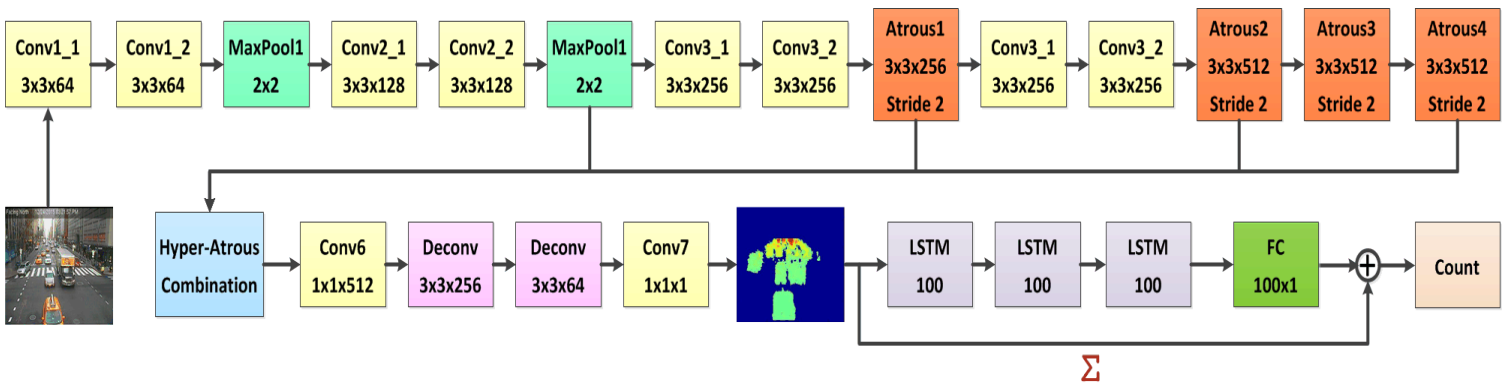
\includegraphics[width=0.9\linewidth]{ChapterThree/fcn_rlstm.png}
    \caption{Architecture of the FCN-rLSTM model (reprinted from \citet{Zhang2017}).}
    \label{fig:fcn_rlstm}
\end{figure}

\Figref{fig:fcn_rlstm} shows the full architecture of this model, from which it can be observed that the convolutional part outputs a density map $\widehat{\mD}$. The density maps are normalized so that the sum of the pixels corresponding to each vehicle sum up to 1 and, therefore, the sum of all pixels in the density map sup to the total number of vehicles in the frame. Thus, the final predicted count $\widehat{y}^{(t)}$ is the result of this sum plus a residual provided by a recurrent neural network, which aims to correct the predicted count by leveraging information from the previous frames.

Training this model implies that each input frame $\mX^{(t)}$ is annotated with the corresponding ground-truth density map $\mD^{(t)}$ and vehicle count $y^{(t)}$. The loss function is defined as:
\begin{equation}
    L(\vtheta) = \frac{1}{n} \sum_{i=1}^{n} ||\widehat{\mD}^{(t)}_i - \mD^{(t)}_i||^2 + \frac{\lambda_c}{n} \sum_{i=1}^{n} ||\widehat{y}^{(t)}_i - y^{(t)}_i||^2,
\end{equation}
where $\lambda_c > 0$ is a hyperparameter controlling the relative weight of the vehicle counting loss, and the dependency of $\widehat{\mD}^{(t)}_i$ and $\hat{y}^{(t)}_i$ on the network parameters $\vtheta$ is omitted to ease the notation.

\subsection{Combining MDAN and FCN-rLSTM}
\label{sec:mdan_fcn_rlstm}
We now explore several possibilities to combine MDAN and FCN-rLSTM into a single model capable of accurately counting vehicles in images from a target camera, provided that at training time we only have access to annotated data from other cameras and unlabeled data from the target.

\subsubsection{Non-Temporal model}
The non-temporal model uses a sub-network in the FCN-rLSTM model as its backbone. It consists in a simplification of this, by not using LSTMs or making any other consideration on the temporal or sequential nature of the data. Figure \ref{fig:non_temporal_model} shows the architecture of the non-temporal model.

\begin{figure}[!ht]
    \centering
    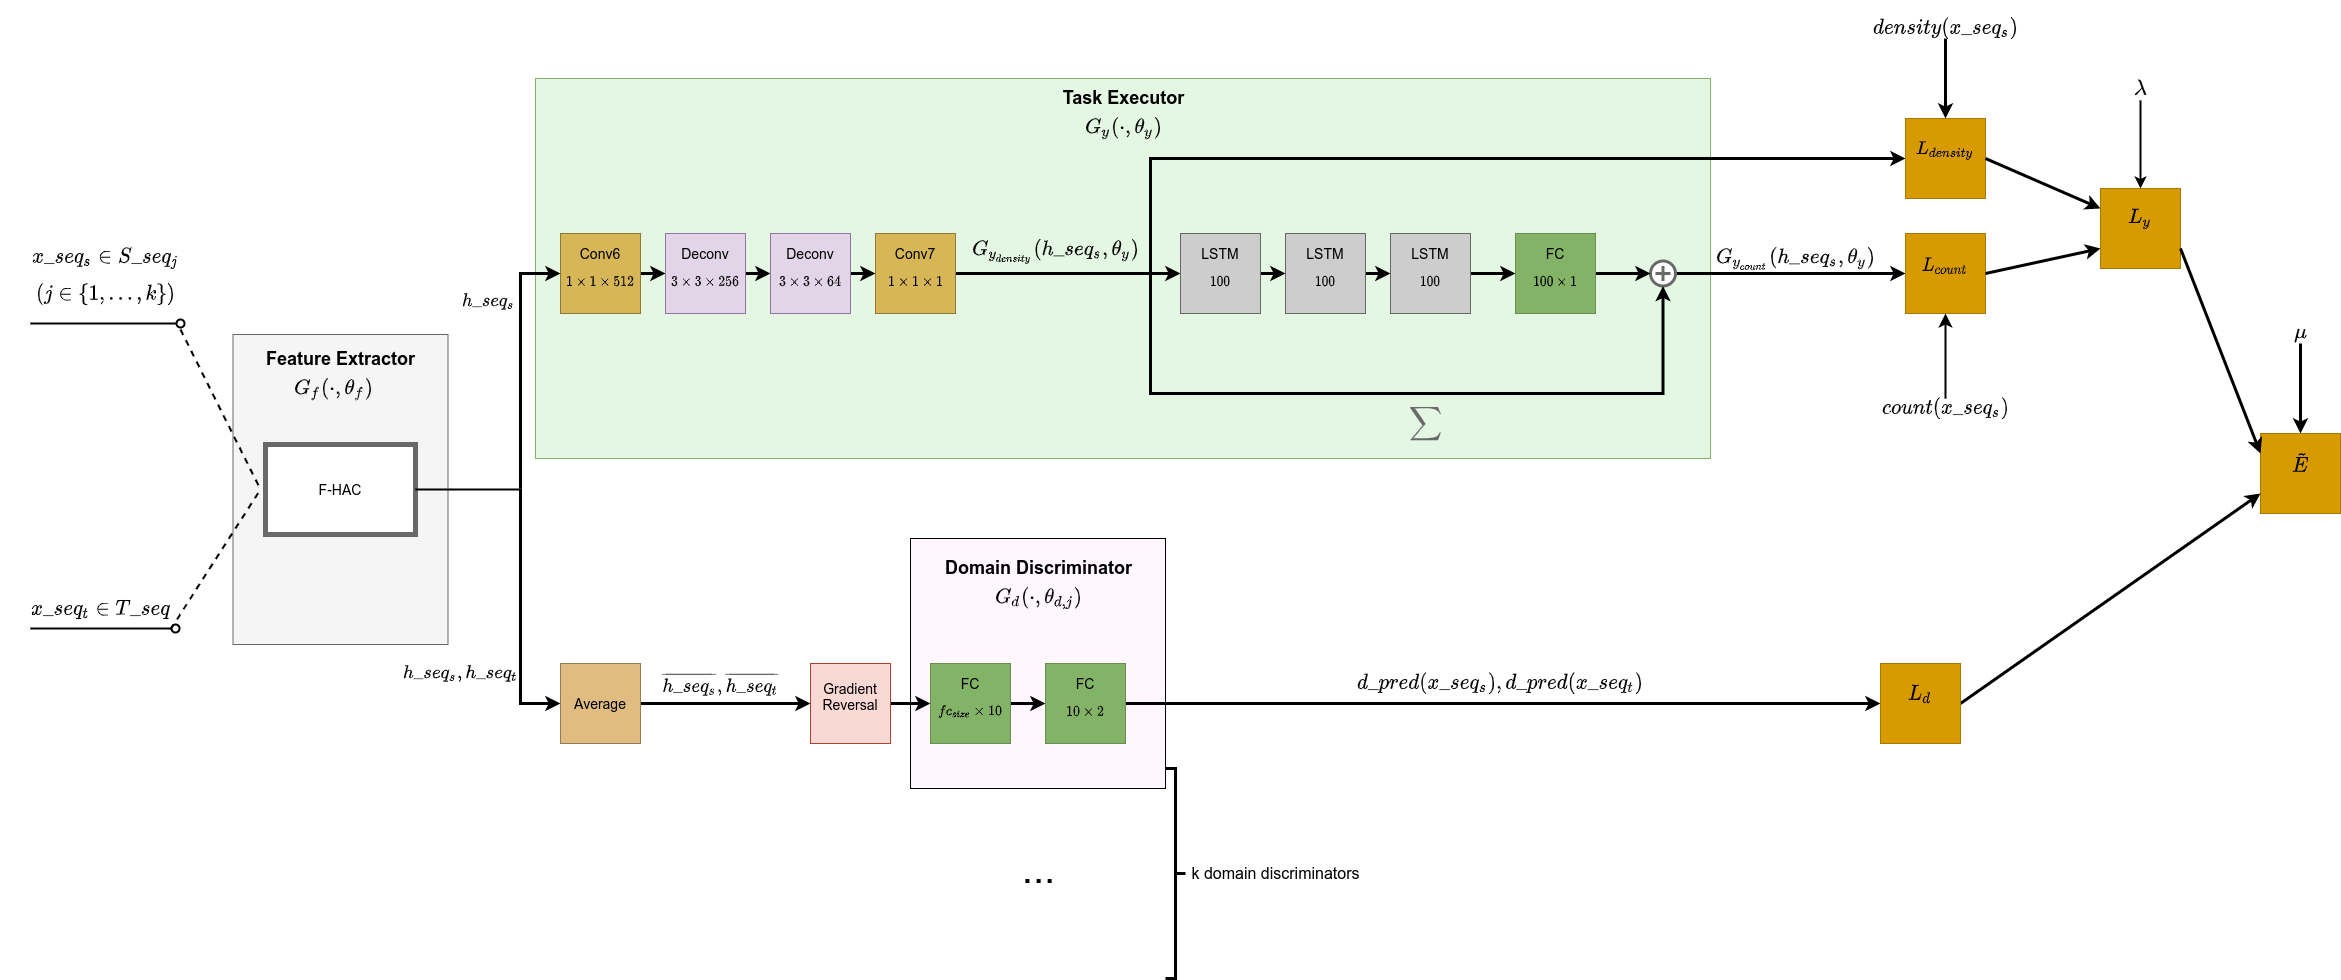
\includegraphics[width=1.0\textwidth]{ChapterThree/non_temporal.png}
    \caption{Non-Temporal model. Reprinted from \citet{ThesisFrancisco}.}
    \label{fig:non_temporal_model}
\end{figure}

The component F-HAC in that figure corresponds to all layers of the FCN-rLSTM up to the hyper-atrous combination. It is used as a feature extractor, whereas the rest of the convolutional layers are used for the object counting task. The $k$ domain discriminators consist of two fully connected layers which are preceded by a gradient reversal layer.

This model will be our baseline as we are primarily interested in merging the benefits of DA techniques and sequential modeling.

\subsubsection{SingleLSTM model}
The SingleLSTM model uses the whole FCN-rLSTM model for the desired regression task, but the domain discriminators are still non-sequential, as shown in \Figref{fig:temporal_regress_model}. Thus, in this model, the domain discrimination task only takes into account the domain-specific information provided by each frame individually and does not account for the domain-specific temporal dynamics that may exist.

\begin{figure}[h!]
    \centering
    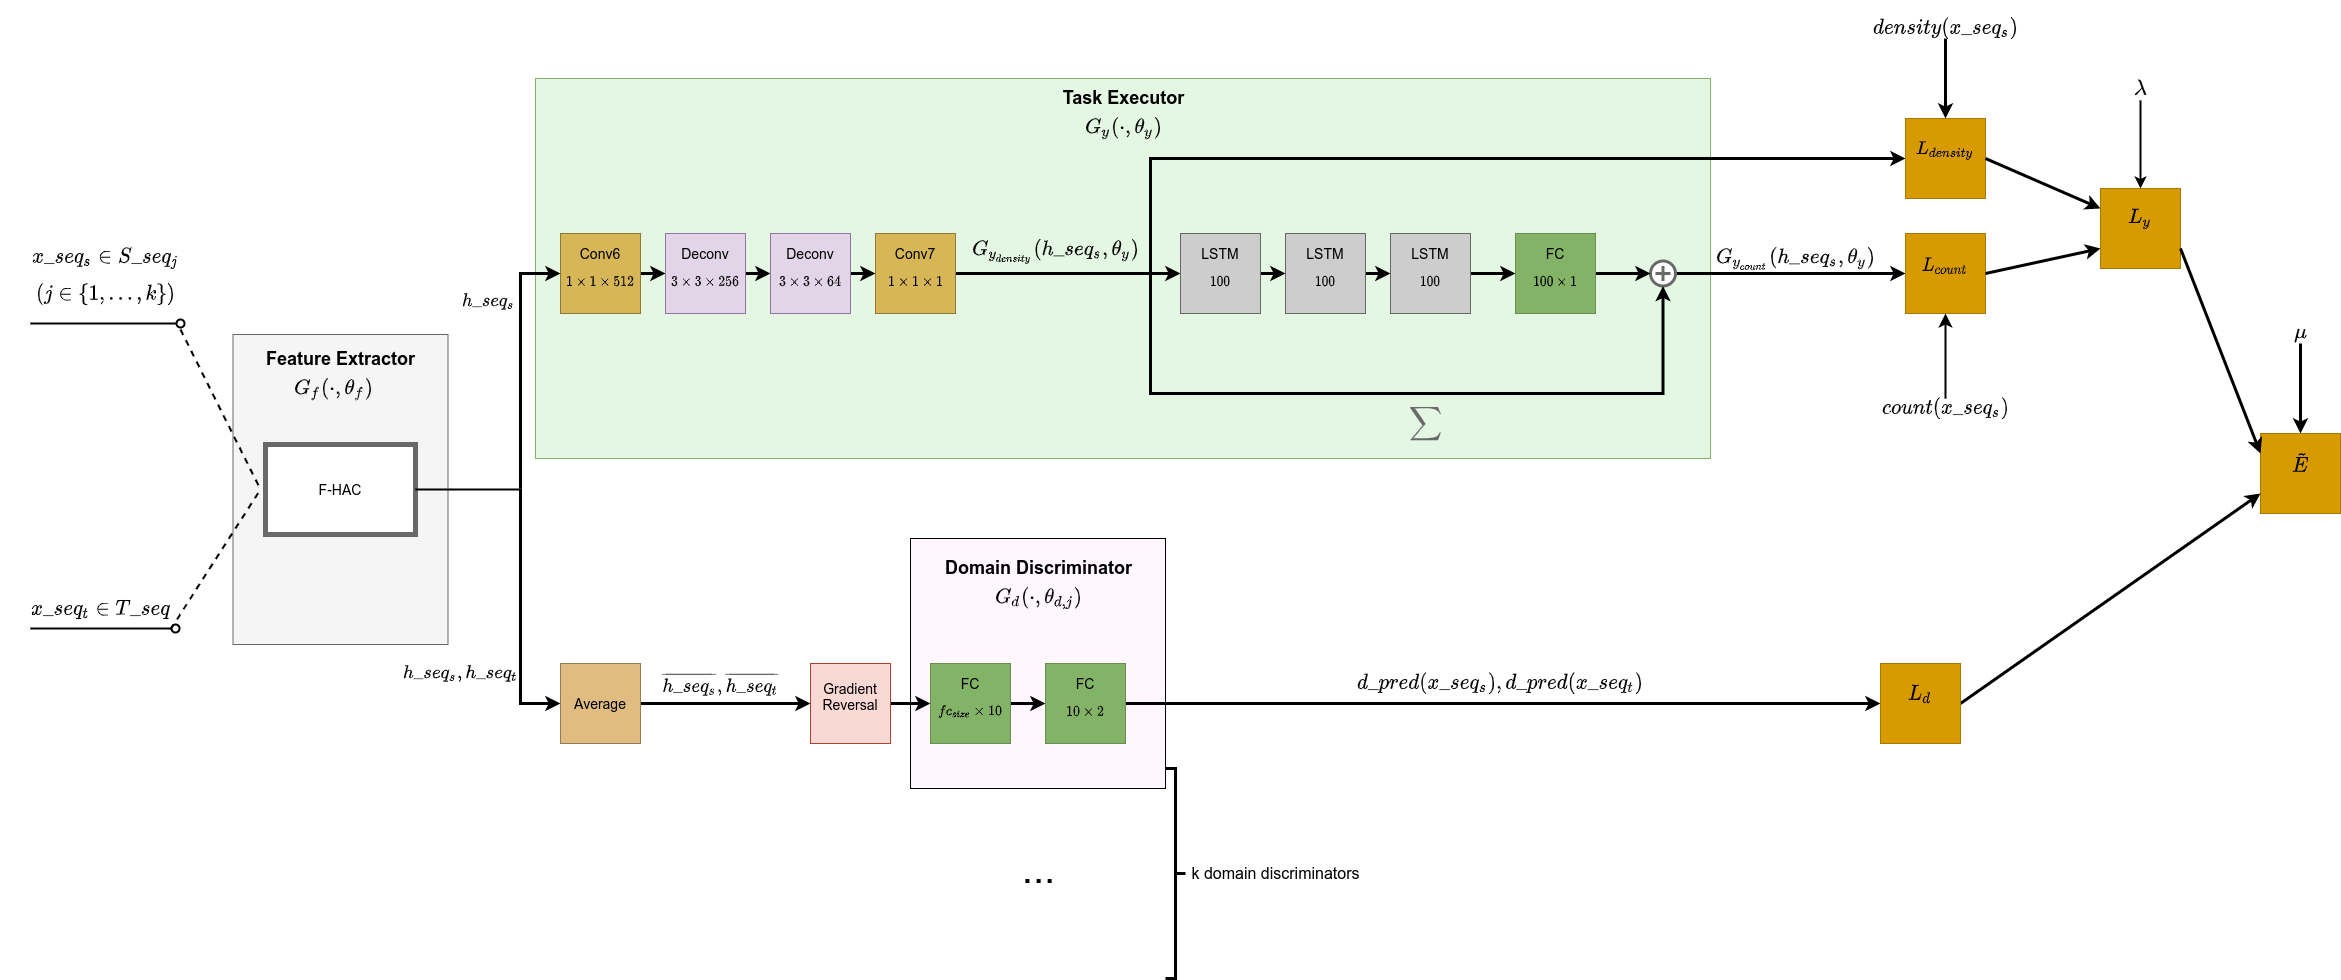
\includegraphics[width=1.0\textwidth]{ChapterThree/temporal_regress.png}
    \caption{Temporal regression model. Reprinted from \citet{ThesisFrancisco}.}
    \label{fig:temporal_regress_model}
\end{figure}

\subsubsection{DoubleLSTM model}
The DoubleLSTM model overcomes the limitations of the SingleLSTM model by incorporating three LSTM layers in each domain discriminator. These aim to learn the domain-specific temporal dynamics that might be helpful for the discrimination task. The schematic is in \Figref{fig:double_temporal_model}.

\begin{figure}[!ht]
    \centering
    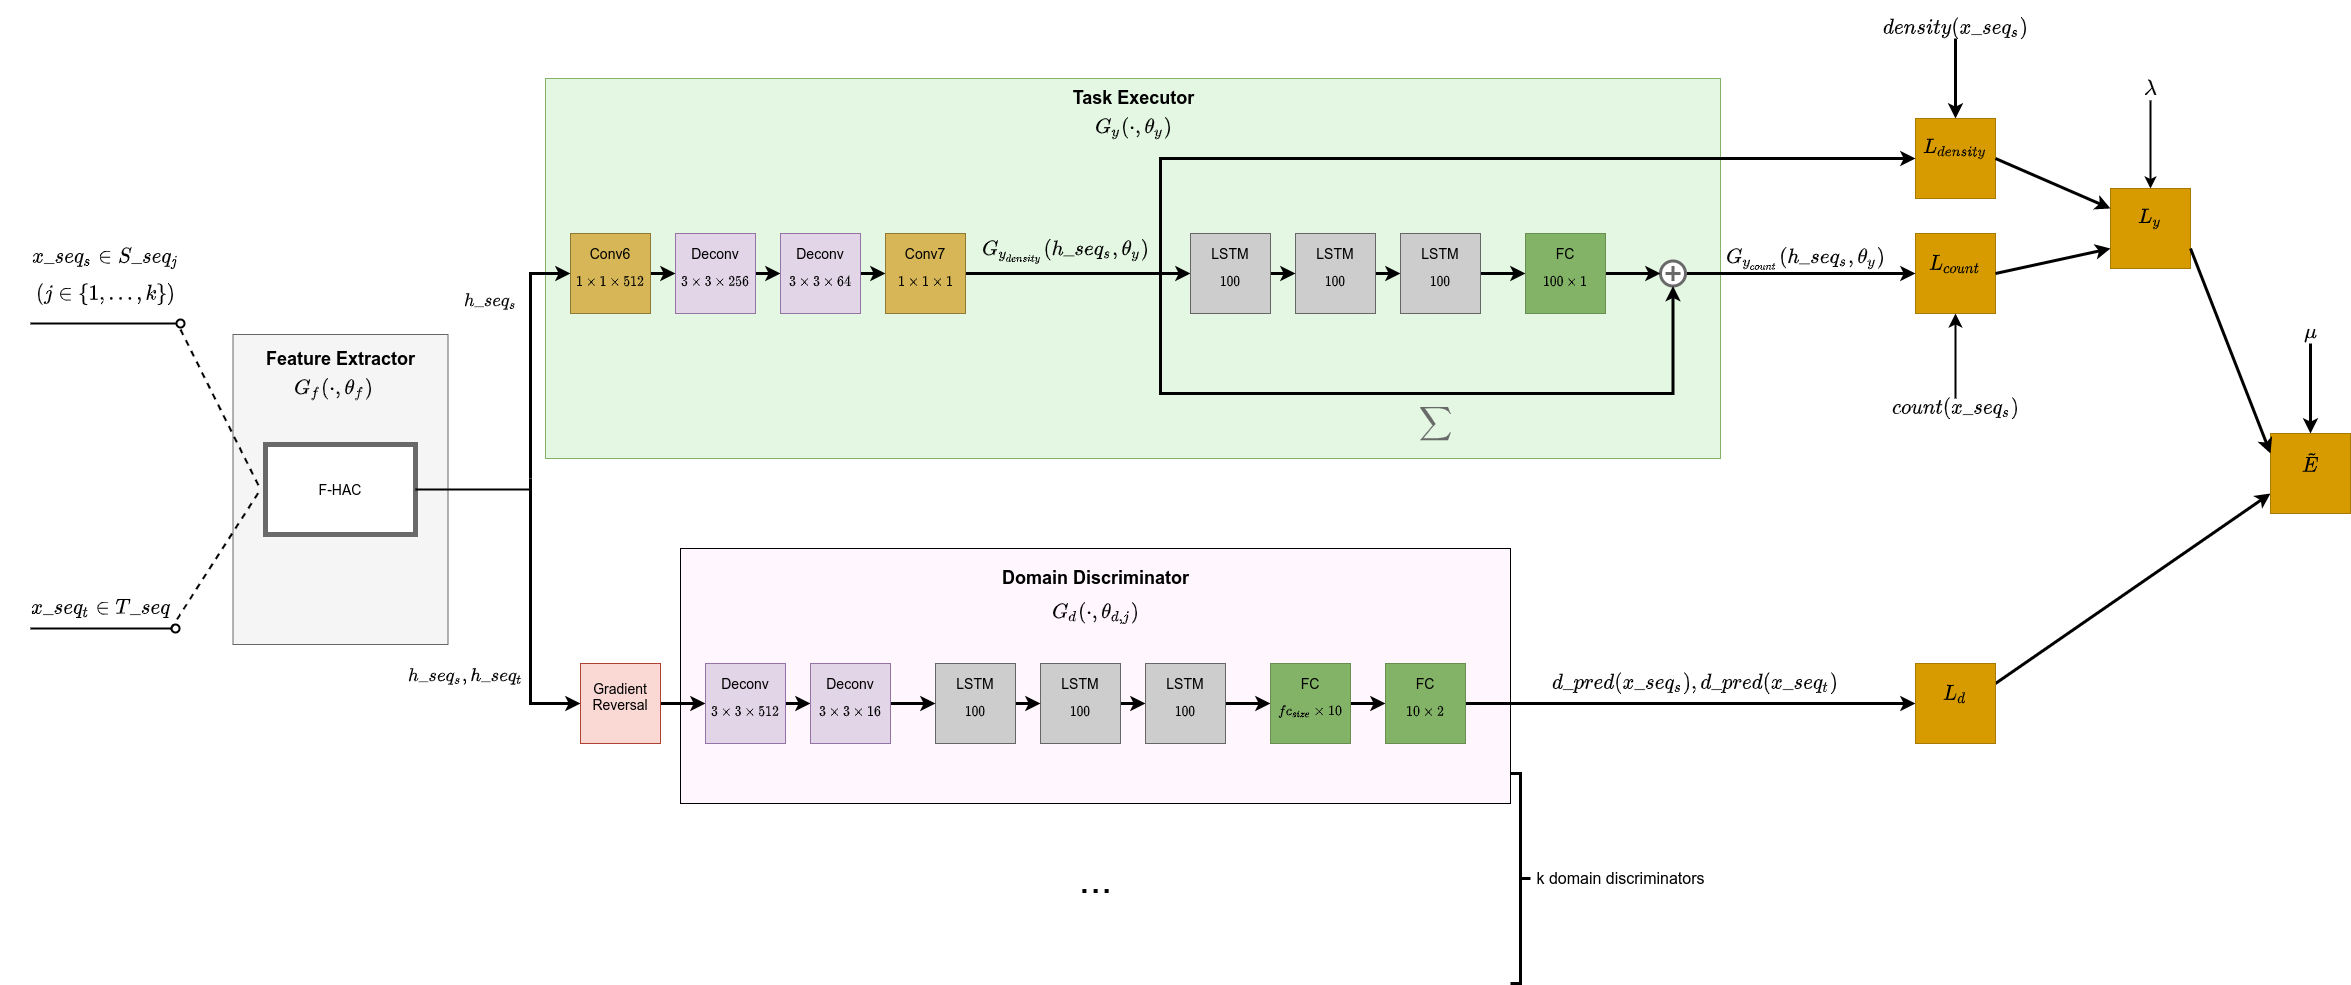
\includegraphics[width=1.0\textwidth]{ChapterThree/double_temporal.png}
    \caption{Double-Temporal model. Reprinted from \citet{ThesisFrancisco}.}
    \label{fig:double_temporal_model}
\end{figure}

\subsubsection{CommonLSTM model}
An alternative to the DoubleLSTM model is to extract temporal features that are common to the desired object counting task and to the domain discrimination task. This is accomplished by the CommonLSTM model, which pushes the domain discriminators after the LSTMs and just before the final fully connected layer, as shown in \Figref{fig:common_temporal_model}.

\begin{figure}[!ht]
    \centering
    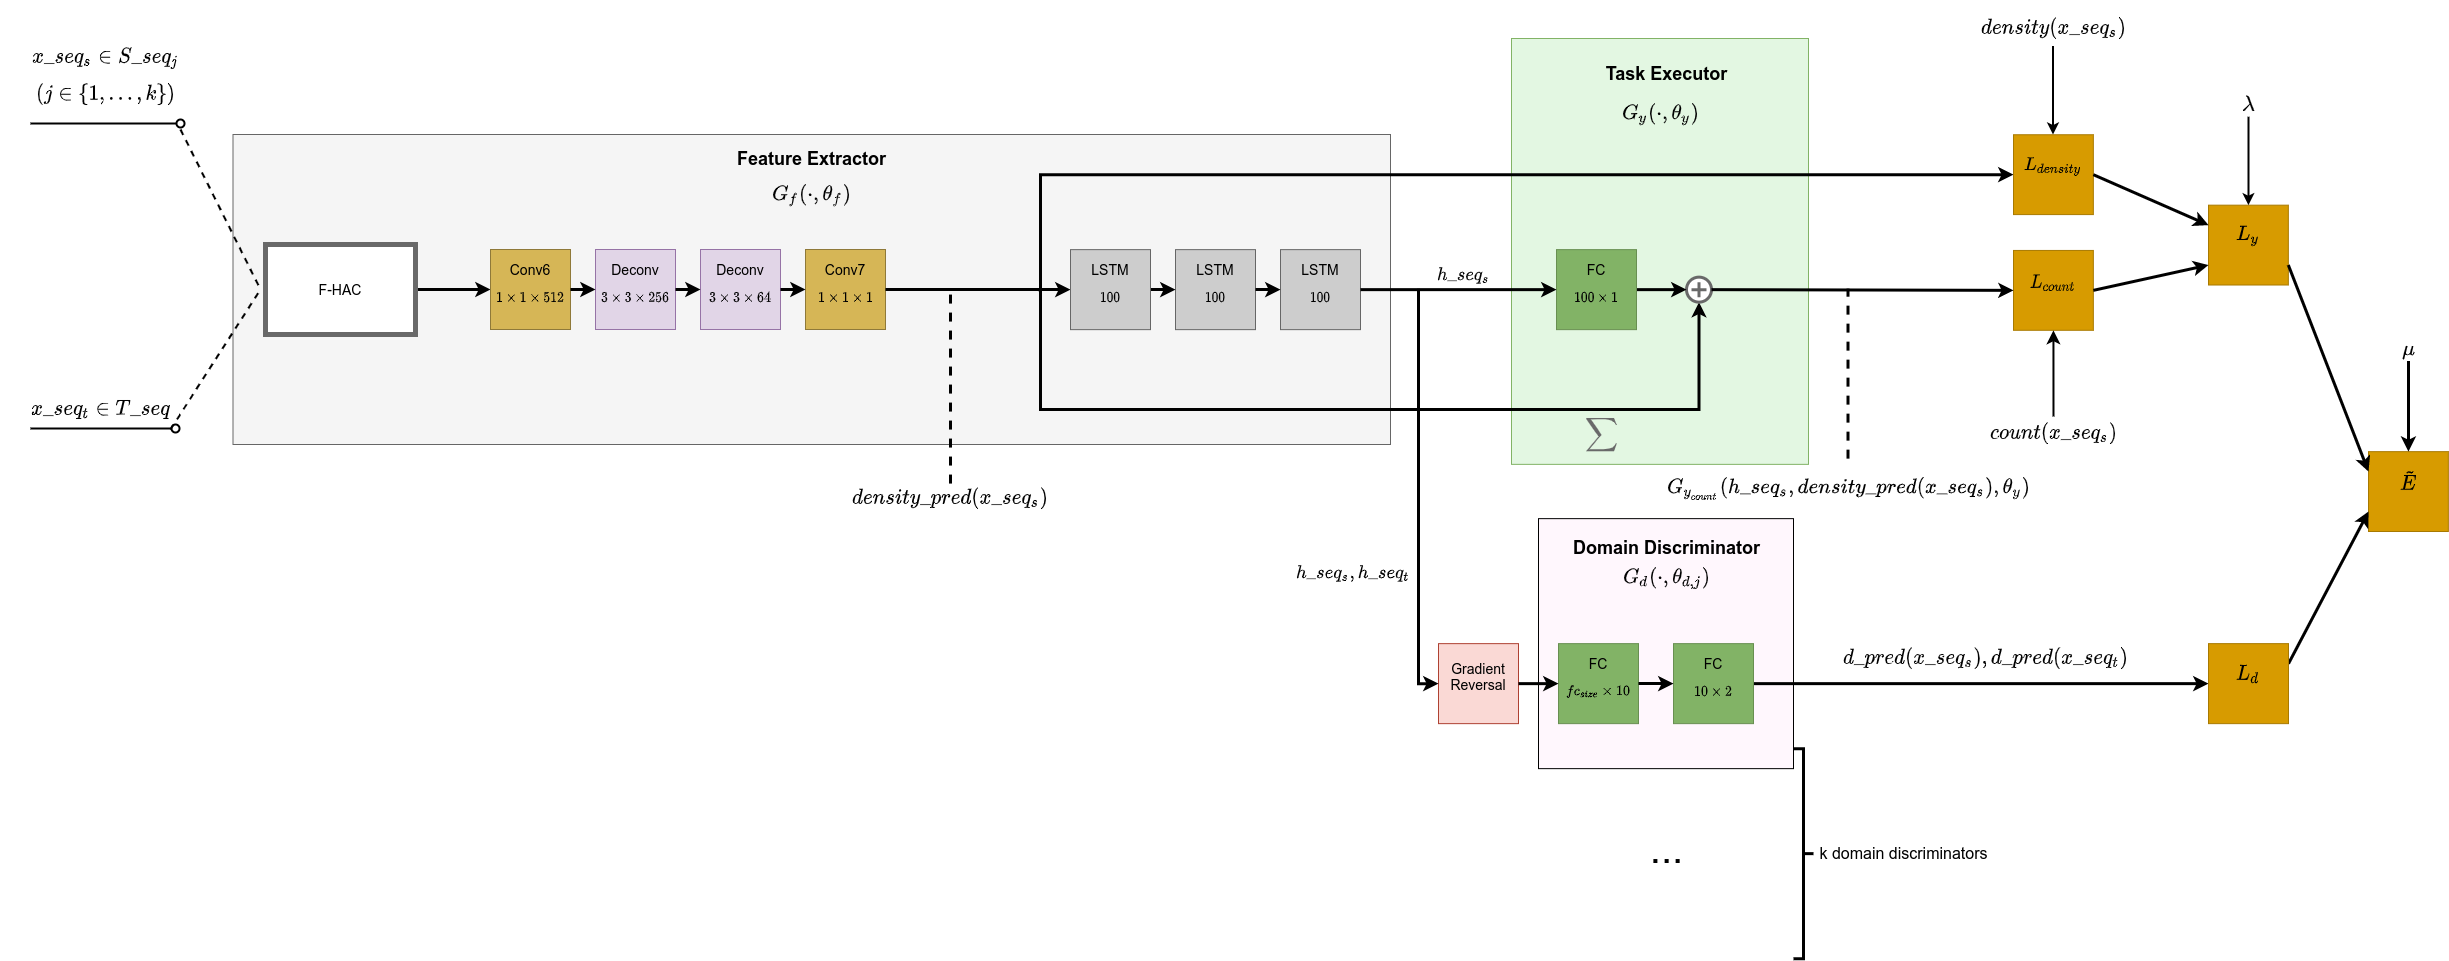
\includegraphics[width=1.0\textwidth]{ChapterThree/common_temporal.png}
    \caption{Common-Temporal model. Reprinted from \citet{ThesisFrancisco}.}
    \label{fig:common_temporal_model}
\end{figure}

This model is fundamentally different from all previous ones since here the feature space where domain-invariance is promoted happens much later in the network. Specifically, the density maps $\widehat{D}$ are a few layers earlier, so they should not be very much affected by the domain-invariance constraint. This might have a beneficial effect on the performance since density maps are defined by the positions in the image where vehicles appear. Since these positions depend on the shape of the street that each camera is capturing, domain-invariant density maps will certainly be inaccurate.

\subsubsection{Overview}

All the proposed models have specific strengths and weaknesses that would make them suitable for certain scenarios and unlikely to show a good performance in others. Here, we anticipate a few of those scenarios.

If the video frame rate is low compared to the objects speed, the number of objects in a given frame is not a good predictor for the number of objects in a subsequent frame. In this setting, the non-temporal model is ideal, as it does not make any temporal consideration. In this case, using a temporal model would have a likely harmful effect on the model performance.

If the frame rate is sufficiently high and the temporal dynamics in the target domain are close to the dynamics in the sources, the SingleLSTM model is likely the best choice. By using an LSTM for the task executor but none for the domain discriminators, it will be able to make small adjustments in the predicted object count and avoid the unnecessary computational cost introduced by having a sequential model in the domain discriminator.

When there is a strong correlation in the object count in consecutive video frames and the dynamics in the target domain are dissimilar to the sources, it may be beneficial to employ sequential models in both the task executor and domain discriminators. Thus, DoubleLSTM and CommonLSTM models are likely to outperform the remaining. Their approach differs, as DoubleLSTM model uses an LSTM network for the task executor and another one for each domain discriminator, whereas CommonLSTM includes an LSTM network in the feature extractor. As the common-temporal model will not enforce similarity between the predicted density maps as much as the double-temporal version, it is probably the best choice when the density maps of the target domain differ significantly from the sources.

\subsection{Experiments}

\subsubsection{Experimental protocol}

We will run experiments with the domain adaptation models presented in \Secref{sec:mdan_fcn_rlstm}. Additionally, we will use models FCN-HA and FCN-rLSTM as baselines, which do not employ any technique to tackle domain shift. The former is a subnetwork of the latter consisting of all layers excluding the LSTM network, i.e.\ it coincides with the Non-Temporal model when its domain discriminator is removed. Therefore, it does not account for any temporal correlations between consecutive frames.

In every experiment, assume we have $k+1$ domains $\gD_1, \gD_2,...,\gD_{k+1}$. In a domain adaptation scenario, we do $k+1$ runs, so that in run number $t$, domain $\gD_t$ will be chosen as the target domain and all the others will be source domains. For each experiment, we have computed results in both unsupervised and semi-supervised settings, described below:

\begin{itemize}
    \item Unsupervised: In this case, we do not have a validation dataset, and, for each run $t$, we calculate the testing results with the model we obtained at the end of the training epochs, for all the samples extracted from domain $\gD_t$.
    \item Semi-supervised: For semi-supervised results, we have a validation dataset that corresponds to $30\%$ of the samples extracted from target $\gD_t$. We use those samples to select the best model obtained throughout the training epochs. This model is then tested with the remaining $70\%$ of the samples from $\gD_t$.
\end{itemize}

For each dataset, we ran a total of $5$ experiments for the DA models, where we varied the value of hyperparameter $\mu_d$ in the range $[10^{-5}, 10^{-1}]$. Recall that $\mu_d$ controls the weight to give to the domain discrimination loss, relative to the task execution loss.

In all experiments, we train the model for $50$ epochs, using Adam optimizer (\citet{Kingma2014}) with a learning rate of $10^{-4}$. The adopted evaluation metric is the Mean Absolute Error (MAE) between the predicted object count and the ground truth for each frame.

\subsubsection{UCSDPeds dataset}
\label{sec:da_sensors_ucsdpeds}

UCSDPeds (\citet{Chan2008}) is a crowd counting dataset that contains videos of pedestrians on University of California, San Diego, walkways, taken from a stationary camera in two different viewpoints. All videos are 8-bit grayscale, with dimensions $158 \times 238$ at a $2$ frames per second rate. For each video frame, the dataset has a mask indicating the region of interest in the image and another file indicating the coordinates of the central point of every person in the frame.

Each camera point of view corresponds to a domain in our experiments, named \textit{vidd} and \textit{vidf}. Figures \ref{fig:ucsdpeds_vidd} and ´\ref{fig:ucsdpeds_vidf} show examples of frames in each one of the two domains.

\begin{figure}[!ht]
    \centering
    \begin{minipage}[b]{0.4\textwidth}
        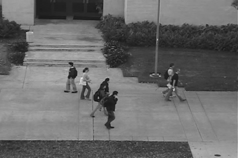
\includegraphics[width=\textwidth]{ChapterThree/vidd_example.png}
        \caption{Domain \textit{vidd} from the UCSDPeds dataset.}
        \label{fig:ucsdpeds_vidd}
    \end{minipage}
    \hfill
    \begin{minipage}[b]{0.4\textwidth}
        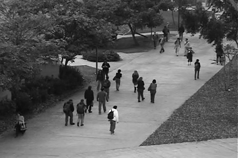
\includegraphics[width=\textwidth]{ChapterThree/vidf_example.png}
        \caption{Domain \textit{vidf} from the UCSDPeds dataset.}
        \label{fig:ucsdpeds_vidf}
    \end{minipage}
\end{figure}

Table \ref{tab:ucsdpeds_domains} shows the mean and standard deviation for the number of people in a frame, for each domain. There is a strong target shift between domains as the mean number of people in domain \textit{vidf} is more than $4$ times higher than the mean number of people in domain \textit{vidd} and, therefore, the DA task is challenging for this dataset.

\begin{table}[!ht]
    \centering
    \begin{tabular}{c| c c}
        & mean & std.\ dev.\  \\
        \hline
        \textit{vidd} & 6.448 & 3.089\\
        \textit{vidf} & 27.570 & 7.393 \\
    \end{tabular}
    \caption{Mean number of people and respective standard deviation for each domain in the UCSDPeds dataset.}
    \label{tab:ucsdpeds_domains}
\end{table}

For each frame, we computed its density map, by placing a $15 \times 8$ Gaussian kernel with sum $1$ on the center of each person. Figure \ref{fig:ucsdpeds_density_map} shows an example of a density map, where the Gaussian kernel around each person is shown in red. The region of interest is also indicated in the figure. As we had only $800$ frames in each domain, we performed data augmentation by adding the mirrored image of each frame to the dataset.

\begin{figure}[!ht]
    \centering
    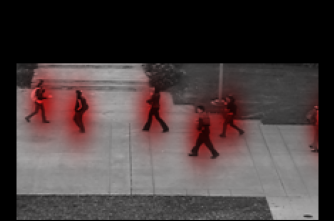
\includegraphics[width=0.75\textwidth]{ChapterThree/ucsdpeds_density_map.png}
    \caption{Sample density map for the UCSDPeds dataset.}
    \label{fig:ucsdpeds_density_map}
\end{figure}

\subsubsection{WebCamT dataset}
\label{sec:da_sensors_webcamt}

WebCamT (\citet{Zhang2017b}) is a vehicle counting dataset that contains city camera videos, taken from a stationary camera in different points of the city of New York. All videos are in color, with dimensions $240 \times 352$, at a $1$ frame per second rate. Every frame in the dataset has a ground truth file with annotations that indicate the center of each vehicle and also its bounding box.

There are $14$ cameras that cover multiple scenes, camera perspectives, congestion states, and weather conditions. We chose four cameras from those $14$ to correspond to our domains. Each of those four cameras had a number of videos, from which we selected $1000$ frames. The frames were selected consecutively, so that if frames $f_1$ and $f_2$ from the same video $V$ were selected, then every frame between $f_1$ and $f_2$ in video $V$ was also selected.

Figures \ref{fig:webcamt_511}-\ref{fig:webcamt_846} show examples of frames in each of the four domains. Table \ref{tab:webcamt_domains} shows the mean and standard deviation for the number of vehicles in a frame, for each domain. As it is possible to observe, the mean number of vehicles in each frame differs significantly across domains, being more than three times larger in domain \textit{691} than in domain \textit{846}. Hence, there is significant target shift in this dataset and, consequently, the covariate shift assumption does not hold.

\begin{figure}[!ht]
    \centering
    \begin{minipage}[b]{0.4\textwidth}
        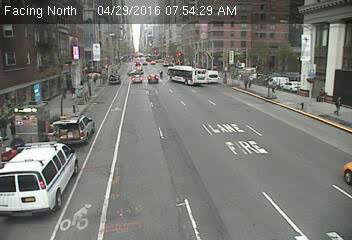
\includegraphics[width=\textwidth]{ChapterThree/511_example.png}
        \caption{Domain \textit{511} from WebCamT dataset.}
        \label{fig:webcamt_511}
    \end{minipage}
    \hfill
    \begin{minipage}[b]{0.4\textwidth}
        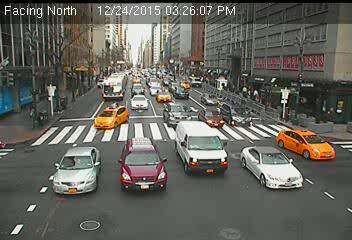
\includegraphics[width=\textwidth]{ChapterThree/551_example.png}
        \caption{Domain \textit{551} from the WebCamT dataset.}
        \label{fig:webcamt_551}
    \end{minipage} \\
    \vspace{1cm}
    \begin{minipage}[b]{0.4\textwidth}
        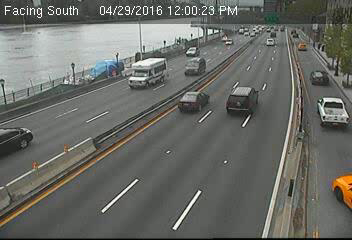
\includegraphics[width=\textwidth]{ChapterThree/691_example.png}
        \caption{Domain \textit{691} from the WebCamT dataset.}
        \label{fig:webcamt_691}
    \end{minipage}
    \hfill
    \begin{minipage}[b]{0.4\textwidth}
        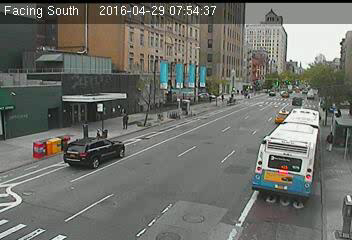
\includegraphics[width=\textwidth]{ChapterThree/846_example.png}
        \caption{Domain \textit{846} from the WebCamT dataset.}
        \label{fig:webcamt_846}
    \end{minipage}
\end{figure}

\begin{table}[!ht]
    \centering
    \begin{tabular}{c| c c}
        & mean & std.\ dev.\  \\
        \hline
        \textit{511} & 12.039 & 6.32 \\
        \textit{551} & 18.362 & 4.21 \\
        \textit{691} & 25.470 & 10.738 \\
        \textit{846} & 6.873 & 2.477 \\
    \end{tabular}
    \caption{Mean number of vehicles and respective standard deviation for each domain in the WebCamT dataset.}
    \label{tab:webcamt_domains}
\end{table}

After extracting each frame from the videos, we computed its density map by placing a $4\times4$ Gaussian kernel with sum $1$ on the center of each car. We then had to resize the frames and density to maps to size $120\times 176$ so that we could deal with speed and memory constraints. Figure \ref{fig:webcamt_density_map} shows an example of a density map in a resized frame, where the Gaussian kernel around each car is shown in red.

\begin{figure}[!ht]
    \centering
    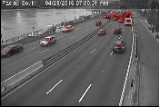
\includegraphics[width=0.75\textwidth]{ChapterThree/webcamt_density_map.png}
    \caption{Sample density map for the WebCamT dataset.}
    \label{fig:webcamt_density_map}
\end{figure}

\subsection{Choice of optimization problem}

The DA task for the UCSDPeds dataset is single source, so there is no choice to be made regarding the combination of source domains. In this setting, the MDAN model boils down to the original adversarial DA algorithm proposed by \citet{Ganin2015}, where one single domain discriminator is used to distinguish between source and target samples.

In the WebCamT dataset, we have three different source domains, so this is a multi-source scenario. As discussed in \Secref{sec:da_sensors_mdan}, we consider three possible optimization problems for our DA models to solve, namely hard-max, soft-max, and average. \Tableref{table:optimization_experiments} shows results for each of our models on these formulations, evaluated in an unsupervised setting. These suggest that averaging tends to perform better than the other two approaches in this dataset. This is somewhat intuitive: given the wide range of values for the mean number of vehicles in each frame across domains, it would be likely for one source domain to show a significantly higher loss than the others. If we use any of the other two optimization problems, our models would dedicate an outweighed importance to the hardest source domain, disregarding the remaining. For this reason, we shall adopt the averaging formulation in all subsequent experiments.

\begin{table}[!ht]
    \centering
    \begin{tabular}{ c | c  c  c }
        & Hard-max & Soft-max & Average\\
        \hline
        Non-Temporal & 18.15 & 11.16 & \textbf{9.91}  \\
        SingleLSTM & 10.54 & \textbf{9.33} & 11.10  \\
        DoubleLSTM & 9.59 & 7.73 & \textbf{6.14} \\
        CommonLSTM & \textbf{9.85} & 12.07 & 10.22 \\
    \end{tabular}
    \caption{Comparison of different optimization problems. The values indicate the average MAE count across domains in the WebCamT dataset. The experiments were run with $\mu_d=10^{-3}$. }
    \label{table:optimization_experiments}
\end{table}

\subsection{Unsupervised setting}

\Tableref{table:results_unsup} shows the results in the unsupervised setting for both datasets. For each domain, the best MAE obtained with different values of $\mu_d$ is shown.
\begin{table}[!ht]
    \centering
    \begin{tabular}{ c | c  c : c | c  c  c  c : c}
        \multicolumn{1}{c|}{} & \multicolumn{3}{c|}{UCSDPeds} & \multicolumn{5}{c}{WebCamT} \\

        & \textit{vidd} & \textit{vidf} & Avg & \textit{511} & \textit{551} & \textit{691} & \textit{846} & Avg\\
        \hline
        FCN-HA & 15.23 & 7.14 & 11.19 & \textbf{5.01} & \textbf{2.58} & 17.22 & 4.67 & 7.37\\

        FCN-rLSTM & 11.04  & 5.98 &  8.51 & 6.26 & 8.79 & 13.63 & 6.31 & 8.75\\

        Non-Temporal & \textbf{6.24} & 22.52 & 14.38 & 9.63 & 3.50 & 18.27 & 5.58 & 9.85 \\

        SingleLSTM & 7.75 & 9.07 & 9.32 & 6.58 & 5.10 & 15.26  & 9.55 & 10.53 \\

        DoubleLSTM & 8.04 & \textbf{3.89} & 6.49 & 5.01 & 4.58 & 10.97 & \textbf{3.03} & \textbf{6.15}\\

        CommonLSTM & 6.83 & 4.80 & \textbf{6.18} & 6.11 & 5.55 & \textbf{10.51} & 3.56 & 8.15 \\

    \end{tabular}
    \caption{MAE count per domain in UCSDPeds and WebCamT datasets (unsupervised setting). Column Avg indicates the average MAE count across domains.}
    \label{table:results_unsup}
\end{table}

In UCSDPeds, CommonLSTM showed the best results, followed by DoubleLSTM. In fact, any LSTM-based model showed a better average performance than any model where LSTMs are absent. This validates our initial hypothesis that making temporal considerations would significantly improve the accuracy. When it comes to the comparison between DA models and non-DA models, we can verify that DA models performed better, as models DoubleLSTM and CommonLSTM showed the best results for average MAE count. Still, in this case, the advantage of promoting domain-invariant representations is not as clear as the advantage of leveraging temporal information. For example, the Non-Temporal model, that includes a domain discriminator, showed worse results than FCN-rLSTM.

In WebCamT, even though the double-temporal showed the best results, the second best was the FCN-HA, a model that does not make any temporal consideration. We also could not verify a marked difference in the average MAE count of the DA and non-DA methods. These observations ascertain that it is not enough to apply domain adaptation or consider the temporal nature of data to obtain good results. Thus, the careful design of models and its integration with the two mentioned techniques is essential.

We find that the model with the most balanced performance across domains and datasets was the DoubleLSTM as its MAE count in a given domain was always in the top-3. This observation coupled with the fact that the DoubleLSTM was also the model with the best average MAE count in UCSDPeds and the second best in WebCamT allows us to conclude that this method was the best-performing overall.

Results regarding the sensitivity to the hyperparameter $\mu_d$ are shown in \Figref{fig:lambda_d_unsup}.

\begin{figure}[!ht]
    \begin{subfigure}{.5\textwidth}
        \centering
        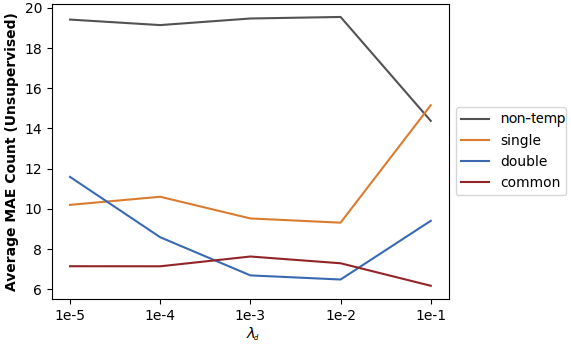
\includegraphics[width=0.95\textwidth]{ChapterThree/ucsdpeds_unsupervised.png}
        \caption{UCSDPeds}
    \end{subfigure}
    \begin{subfigure}{.5\textwidth}
        \centering
        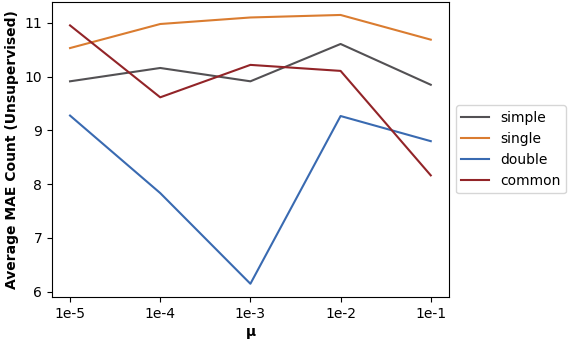
\includegraphics[width=0.95\textwidth]{ChapterThree/webcamt_unsupervised.png}
        \caption{WebCamT}
    \end{subfigure}
    \caption{Average MAE count across domains for each $\mu_d$ in the unsupervised setting in UCSDPeds and WebCamT datasets.}
    \label{fig:lambda_d_unsup}
\end{figure}

This plot confirms that the DoubleLSTM model was the best-performing in the WebCamT dataset and is at least comparable to CommonLSTM in UCSDPeds. Setting $\mu_d = 10^{-3}$ achieves close to optimal performance for all models in both datasets, except for Non-Temporal in UCSDPeds and CommonLSTM in WebCamT, whose performance improves significantly for larger values of $\mu_d$.

\subsection{Semi-supervised setting}

\Tableref{table:results_semisup} shows the results in the semi-supervised setting for both datasets. Like before, the best MAE obtained with different values of $\mu_d$ is shown.

\begin{table}[!ht]
    \centering
    \begin{tabular}{ c | c  c : c | c  c  c  c : c}
        \multicolumn{1}{c|}{} & \multicolumn{3}{c|}{UCSDPeds} & \multicolumn{5}{c}{WebCamT} \\
        & \textit{vidd} & \textit{vidf} & Avg & \textit{511} & \textit{551} & \textit{691} & \textit{846} & Avg\\
        \hline
        FCN-HA & 1.43 & 4.48  & 2.96 & \textbf{2.05} & \textbf{2.59} & 6.56 & 2.394 & \textbf{3.40} \\
        FCN-rLSTM & 2.01 & \textbf{2.07} & 2.04 & 5.40 & 3.49 & 9.15 & 3.54 &  5.39 \\
        \hline
        Non-Temporal & 0.84 & 3.49 & 2.21 & 3.11 & 3.57 & 10.96 & 2.05 & 5.04 \\
        SingleLSTM & 0.94 & 5.07 & 3.00 & 4.24 & 4.39 & 7.03 & \textbf{1.52} & 4.34 \\
        DoubleLSTM & 0.95 & 2.84 & \textbf{1.89} & 4.22 & 4.55 & \textbf{6.46} & 1.58 & 4.27 \\
        CommonLSTM & \textbf{0.88} & 2.61 & 1.94 & 4.23 & 4.54 & 8.67 & 1.63 & 4.98 \\
    \end{tabular}
    \caption{MAE count per domain in UCSDPeds and WebCamT datasets (semi-supervised setting). Column Avg indicates the average MAE count across domains.}
    \label{table:results_semisup}
\end{table}

There is a noticeable difference between these results and those for the unsupervised setting (\Tableref{table:results_unsup}), with the former being significantly better that the latter. As the experiments we ran with the WebCamT had more data and more domains, the resulting models have smaller variance, which caused the difference in accuracy between the two settings not to be as wide as in UCSDPeds.

In UCSDPeds, we can discern the same general remarks we made when we analyzed the unsupervised problem. Models DoubleLSTM and CommonLSTM showed the best performance. Temporal models proved better than non-temporal ones, although in this case, model SingleLSTM had the worst average MAE count. DA models proved, in general, to be better than non-DA models.

For WebCamT, again we were not able to notice a significant difference between the performance of the temporal methods and the non-temporal ones. As we have also verified before, the DA models do not show a marked improvement over the non-DA models for the WebCamT dataset. In fact, in this case, it was a non-temporal, non-DA model, the FCN-HA, that showed the best average MAE count.

Please refer to \citet{ThesisFrancisco} for an extended discussion and further experimental results.

\subsection{Conclusion}

We have proposed several sensible model architectures to solve the problem of domain adaptation for the task of counting objects in videos. All of those result from the combination of two state of the art models, one for the object counting task (FCN-rLSTM) and the other one for multi-source DA (MDAN).

Among the proposed models, it stands out that DoubleLSTM and CommonLSTM showed a significant improvement over the non-DA model FCN-rLSTM in most cases. Models Non-Temporal and SingleLSTM, on the other hand, had a very unsatisfactory performance, by not showing better results than methods FCN-rLSTM and FCN-HA. We have thus verified that integrating domain adaptation with a method does not automatically guarantee better results. Careful considerations on how to divide the previous method between feature extractor and task executor should be made, just like careful deliberations on the domain discriminator design and choice of the hyperparameter $\mu_d$. Unfortunately, informed choices about these become especially difficult in the unsupervised setting, where it is impossible to obtain a direct evaluation of how a given choice will perform on the target domain.

It should also be noted that the results showed an inconsistency in the performance of models across domains. That is, whereas a model performed better in one domain, another model performed better in another. Hence, when applying a model for counting objects in a real world scenario, one should ponder what model to use depending on the characteristics of the particular target domain.

All the previous considerations prove the difficulty of the DA problem, especially when the domain shift is large as was the case in the two datasets we have used in these experiments. This discussion makes a good starting point for the next section, where a novel algorithm for unsupervised multi-source DA is presented.

\section{Tackling multi-source domain adaptation with optimism and consistency}
\label{sec:modafm}

\subsection{Introduction}
\label{sec:modafm_intro}
The ability of deep neural networks to learn rich feature representations and the recent surge of adversarial learning techniques have led to numerous approaches that resort to an adversarial objective to learn those representations. The adversary is usually implemented with a domain discriminator network (\citet{Ganin2015}), which aims to discriminate samples between source and target domains, and is jointly trained with the feature extractor and task classifier through a minimax game. Other models resort to the minimization of  distribution dissimilarity metrics between the target and source feature distributions (\citet{DeSIRe, Guo2018}). It is known, however, that if the learned features violate the covariate shift assumption, domain-invariant features shall deteriorate the generalization performance of the model on the target domain (\citet{Zhao2019}) -- a problem that we refer to as \newterm{the curse of domain-invariant representations}. Addressing this issue in the unsupervised setting is challenging, although some strategies have been proposed. \citet{Pei2018} use a domain discriminator per class and the probability output of the task classifier as attention weights for the discriminator. \citet{Sebag2019} introduce a loss term that repulses unlabeled examples from the labeled ones whenever the classifier has low confidence on classifying the unlabeled examples. Thus, both methods depend on the classifier to make correct predictions on the target samples early in the training. Here, we avoid this issue by employing a consistency loss, together with a minimum confidence threshold, that enforces agreement on the class predictions for original and augmented target samples.

Our contributions in this section are summarized as follows: i) we present a corollary of the theoretical results from \citet{BenDavid2010} which motivates our methodology (\Secref{sec:moda_motivation}); ii) we present our multi-source adversarial model which learns the distribution weights for each source domain jointly with all remaining parameters and following a theoretically-grounded mildly optimistic approach (\Secref{sec:modafm_mixture}); iii) we discuss how a simple consistency regularization technique may help avoid the curse of domain-invariant representations (\Secref{sec:modafm_consistency}); iv) we conduct extensive experiments on benchmark datasets that confirm the effectiveness of the proposed methodologies (\Secref{sec:modafm_experiments}).

\subsection{Motivation}
\label{sec:moda_motivation}
\subsubsection{An upper bound on the target risk}

Intuitively, if the source and target domains are similar and the amount of labeled source data is sufficiently large, a classifier trained to reach low empirical error on the source domain will likely achieve a low error on the target domain too. When multiple source domains are available, a combination of their respective data yields the optimal strategy. The following bound, which is a corollary of the results from \citet{BenDavid2010}, formalizes these ideas and enlightens some properties that will be exploited by our approach. For completeness, the proof is provided in Appendix \ref{sec:thm_proof}. In the following, $\Delta$ denotes the $k$-simplex and $\gS_{\valpha}$ is the $\valpha$-weighted mixture of source domains (i.e.\ $\Delta \triangleq \lbrace \valpha \in [0,1]^k: \sum_{j=1}^{k} \alpha_j = 1$ and  $p_{\gS_{\valpha}}(\rvx) \triangleq \sum_{j=1}^{k} \evalpha_j p_{\gS_j}(\rvx)$).

\begin{theorem}
    \label{thm:target_risk_bound}
    Let $\gH$ be a hypothesis class with VC-dimension $d$. Consider an unlabeled set of $n$ samples drawn from the target domain $\gT$ and, for each $j \in \{1,2,...,k\}$, a labeled set of $n/k$ samples drawn from the source domain $\gS_j$. Then, for any $h \in \gH$ and any $\alpha \in \Delta$, with probability at least $1-\delta$ over the choice of samples,
    \begin{equation}
        \label{eq:bound}
        \epsilon_\gT(h) \leq \sum_{j=1}^k \alpha_j \widehat{\epsilon}_{\gS_j}(h) + \frac{1}{2} \widehat{d}_{\gH \Delta \gH}(\gS_\valpha, \gT) + \lambda_\valpha + B_\valpha(\delta) + V(\delta),
    \end{equation}
    where
    \begin{align}
        &B_\valpha(\delta) \triangleq 2\sqrt{\frac{k}{n}\left(2d \log(2(n+1)) + \log\frac{8}{\delta}\right)\sum_{j=1}^k \evalpha_j^2}, \\
        &\lambda_\valpha \triangleq \min_{h \in \gH}\, \sum_{j=1}^k \evalpha_j \epsilon_{\gS_j}(h) + \epsilon_{\gT}(h), \\
        &V(\delta) \triangleq 2 \sqrt{\frac{1}{n} \left( 2d\log(2n) + \log\frac{4}{\delta} \right)}.
    \end{align}
\end{theorem}
This bound is structurally very similar to the one presented in Theorem \ref{thm:da_bound_multi_source} (\citet{Zhao2018}), with two slight differences: i) we work with the (empirical) $\gH \Delta \gH$-divergence between the target and the mixture of source domains directly, instead of upper-bounding it with the convex combination of (empirical) $\gH \Delta \gH$-divergences between the target and each source domain; and ii) we show the dependency of the bound on the quantity $B_\valpha(\delta)$, whose interpretation is given in the following discussion.

\subsubsection{The curse of domain-invariant representations}
\label{sec:modafm_domain_invariance}
If the optimal $\valpha$ was known, a learning algorithm for DA could, in principle, be trained to minimize the first two terms in the bound. For this purpose, it should find a function $g:\gX \mapsto \gZ$ in a set of feature transformations $\gF$ and a classifier $h: \gZ \mapsto \gY$ in $\gH$. The first term in the bound is minimized by training the classifier $h$ on the desired task, using the labeled data from all source domains. The second term is minimized by finding a feature transformation $g$ such that the induced distributions $\gT^g$ and $\gS_\valpha^g$ are similar. This is the main idea exploited by adversarial-based DA algorithms, which use an adversarial objective to match source and target distributions in a latent feature space. The problem with this approach is that it completely overlooks the role of the third term, $\lambda_\valpha$, which corresponds to the minimum possible combined risk of a classifier in $\gH$ on the source and target domains. \citet{Zhao2019} show constructively that a low error on the source domain and domain-invariant features are insufficient to ensure low target risk and may actually have the opposite effect, by increasing $\lambda_\valpha$. Sufficiency is established only under the covariate shift assumption, where the conditional distributions of labels $\ry \in \gY$ given features $\rvz \in \gZ$ are the same across source and target domains and only the marginal distributions of features differ. Since, in the unsupervised DA setting, target labels are not available, imposing or verifying covariate shift is not possible. Moreover, whenever the marginal distributions of labels differ (target shift), a strong enforcement of domain-invariant feature representations necessarily hurts the covariate shift assumption, by imposing the marginals on features to coincide. For this reason, training adversarial-based DA algorithms for many iterations generally yields worse performance (\citet{Zhao2019}). In this work, we show empirically that learning a more robust feature transformation will generally help mitigate this issue.

\subsubsection{Choosing the combination of source domains}
\label{sec:modafm_choose_alpha}
Looking at the first two terms of the learning bound in Theorem~\ref{thm:target_risk_bound} suggests that $\valpha$ could be chosen in an optimistic way, by selecting the source domain in which the sum of the risk of the classifier and the $\gH \Delta \gH$-divergence with respect to the target reaches the lowest value. However, the term $B_\valpha(\delta)$ is proportional to the $\normltwo$-norm of $\valpha$, which is maximum when $\valpha$ is one-hot and minimum when $\evalpha_j = 1/k$, $\forall\, j$. This has an intuitive explanation: choosing a sparse $\valpha$ implies discarding data from the source domains whose component is zero, so the classifier is trained with intrinsically less data and its error tends to increase. This discussion naturally leads to the following formal objective:
\begin{equation}
    \label{eq:formal_obj}
    \min_{\valpha \in \Delta, \, h\in \gH, \, g \in \gF}\; \sum_{j=1}^k \alpha_j\widehat{\epsilon}_{\gS_j}(h \circ g) + \frac{1}{2} \widehat{d}_{\gH \Delta \gH}(\gS_\valpha^g, \gT^g) + \mu ||\valpha||,
\end{equation}~
where $\mu = \mu(\delta) > 0$. This objective contrasts with the idea from \citet{Zhao2018}, where the authors essentially choose to minimize the loss for the hardest source domain at each iteration of the learning algorithm, which is a much more pessimistic approach than ours. In either case, though, the minimum combined risk $\lambda_\valpha$ is uncontrolled and, as discussed in \Secref{sec:modafm_domain_invariance}, this is an issue that must be addressed.

\subsection{Methodology}
\label{sec:modafm_method}

Given the discussion in the previous section, we now explain our method in detail. It basically consists of two major approaches, explained throughout this section.

\subsubsection{Domain adaptation from a dynamic mixture of sources}
\label{sec:modafm_mixture}

We first address the problem of casting the objective~\plaineqref{eq:formal_obj} into a computationally treatable surrogate. As in many recent works in DA, we resort to neural networks to implement $g$ and $h$ and the empirical $\gH \Delta \gH$-divergence is implemented with a domain discriminator network, which aims to distinguish between samples of $\gS_\alpha^g$ and $\gT^g$.\footnote[1]{Theoretically, some care should be taken while designing the architecture of the discriminator to make sure that it parametrizes hypotheses in $\gH \Delta \gH$, but in practice this constraint is dropped. There are similar bounds using the $\gH$-divergence instead \citep{Sebag2019}.} Taking the previous considerations and replacing the intractable empirical risks by the usual classification losses, objective~\plaineqref{eq:formal_obj} is cast as:
\begin{equation}
    \min_{\valpha \in \Delta, \vtheta_g, \vtheta_h} \max_{\theta_d} \; \Big\{ \gL(\valpha, \vtheta_g, \vtheta_h, \vtheta_d) = \gL_\text{class}(\valpha, \vtheta_g, \vtheta_h) - \mu_d \gL_\text{disc}(\valpha, \vtheta_g, \vtheta_d) + \mu_s ||\valpha||^2 \Big\},
\end{equation}
where
\begin{align}
    &\gL_\text{class}(\alpha, \vtheta_g, \vtheta_h) = -\sum_{j=1}^M \alpha_j\E_{\rvz \sim \gS_j^g} \left[\log p(\ry=f_{\gS_j^g}(\rvz) \mid \rvz, \vtheta_h)\right], \\
    %
    &\gL_\text{disc}(\alpha, \vtheta_g, \vtheta_d) = -\E_{\rvz \sim \gS_{\valpha}^g} \left[ \log p(\rd=0 \mid \rvz, \theta_d) \right] - \E_{\rvz \sim \gT^g} \left[ \log p(\rd=1 \mid \rvz, \vtheta_d) \right].
\end{align}
Here, $\vtheta_h$ and $\vtheta_d$ are the parameters of the classifier and domain discriminator networks, respectively, $\mu_d, \mu_s > 0$ are hyperparameters, $\ry \in \gY$ is the categorical r.v. associated with the class label, $f_{\gS_j^g}: \gZ \mapsto \gY$ is the true (multiclass) labeling function for the $j$-th source domain, $\rd$ is a Bernoulli random variable that discriminates source and target domains and the function $g = g(\cdot, \vtheta_g): \gX \mapsto \gZ$ is a neural network, parametrized by $\vtheta_g$, mapping input samples to features. By linearity of expectations and using the fact that $\rvz = g(\rvx, \vtheta_g)$, for input samples $\rvx \in \gX$, we have:
\begin{align}
    \label{eq:loss_class}
    \gL_\text{class}(\valpha, \vtheta_g, \vtheta_h) &\triangleq -\sum_{j=1}^k \alpha_j\E_{\rvx \sim \gS_j} \left[ \log p(\ry=f_{\gS_j}(\rvx) \mid \rvx; \vtheta_g, \vtheta_h) \right], \\
    \allowdisplaybreaks
    \label{eq:loss_disc}
    \gL_\text{disc}(\valpha, \vtheta_g, \vtheta_d) &\triangleq -\sum_{j=1}^k \alpha_j\E_{\rvx \sim \gS_j} \left[ \log p(\rd=0 \mid \rvx; \vtheta_g, \vtheta_d) \right] - \E_{\rvx \sim \gT} \left[ \log p(\rd=1 \mid \rvx; \vtheta_g, \vtheta_d) \right] .
\end{align}
In order to satisfy the constraint $\valpha \in \Delta$, we reparametrize the model using $\alpha = \softmax(\vbeta)$, for an unconstrained parameter $\vbeta \in \sR^k$. Finally, since we assume to have access to labeled datasets $\widehat{\gS}_1,\widehat{\gS}_2,\dots,\widehat{\gS}_k$ from each source domain and to a unlabeled dataset $\widehat{\gT}$ from the target, we may compute empirical estimates of losses \plaineqref{eq:loss_class} and \plaineqref{eq:loss_disc}:
\begin{equation}
    \label{eq:emp_loss_class}
    L_\text{class}(\vbeta, \vtheta_g, \vtheta_h) \approx -\frac{1}{m}\sum_{j=1}^k \frac{\exp(\evbeta_j)}{\sum_{j'} \exp(\evbeta_{j'})} \sum_{(\vx,y) \in \widehat{\gS}_j^{(m)}} \log p(y \mid \vx; \vtheta_g, \vtheta_h),
\end{equation}
\begin{align}
    \label{eq:emp_loss_disc}
    L_\text{disc}(\vbeta, \vtheta_g, \vtheta_d) \approx& -\frac{1}{m}\sum_{j=1}^k \frac{\exp(\evbeta_j)}{\sum_{j'} \exp(\evbeta_{j'})} \sum_{(\vx,y) \in \widehat{\gS}_j^{(m)}} \log p(\rd=0 \mid \vx; \vtheta_g, \vtheta_d) \\
    &-\frac{1}{m}\sum_{\vx \in \widehat{\gT}^{(m)}} \log p(\rd=1 \mid \vx; \vtheta_g, \vtheta_d), \nonumber
\end{align}
where $\widehat{\gS}_j^{(m)}$ and $\widehat{\gT}^{(m)}$ are mini-batches of $m$ examples each from $\widehat{\gS}_j$ and $\widehat{\gT}$, respectively.

It is instructive to compare our approach with MDAN (\citet{Zhao2018}), as that model is the most similar to ours. The bound in \eqref{eq:bound} uses one single $\gH \Delta \gH$-divergence and, therefore, our model comprises one single domain discriminator, which aims to distinguish between the target and the $\valpha$-weighted mixture of source domains. \citet{Zhao2018} use $k$ discriminator networks, i.e.\ one per source domain. More importantly, regarding the choice of $\valpha$, we treat it as one further parameter that can be optimized to minimize the loss. To avoid the objective to collapse into the easiest source domain, as explained in \Secref{sec:modafm_choose_alpha}, we include an extra term that penalizes a sparse $\valpha$. Unlike us, they do not include the sparsity penalization term and choose $\valpha$ to minimize the worst case scenario, by assigning a larger weight to the maximum loss among the $k$ source domains on each training iteration.

\subsubsection{Consistency regularization on the target domain}
\label{sec:modafm_consistency}

Consistency regularization is a key component of many state of the art algorithms in semi-supervised learning. The basic idea is simple: an unlabeled sample and a slightly perturbed version of it should share the same label. Here, this approach is exploited as a sensible heuristic to avoid that domain-invariant features end up hurting the generalization performance of the model on the target domain, as discussed in \Secref{sec:modafm_domain_invariance}.

Specifically, consider a target sample $\vx \in \widehat{\gT}$ and a parametric transformation $\omega: \gX \times \Xi \mapsto \gX$, where $\Xi$ is the space of parameters for the transformation. Further assume that $\omega$ is label-preserving, i.e.\ $f_\gT(\omega(\vx, \xi)) = f_\gT(\vx)$, $\forall\, \vx \in \gX, \, \xi \in \Xi$. If $\omega$ is rich and strong enough, it should spread the transformed target samples over multiple regions of low density under the target distribution, i.e.\ it will produce new domains. Then, by enforcing agreement on the predictions of original and transformed target samples, we are encouraging the model to learn to extract features that generalize well across domains. Moreover, some of the augmented samples may fall within regions of higher density under the distribution of the source domains. If this hypothesis holds, by enforcing agreement on the predictions of original and transformed target samples and low classification error on the source domains, we are indirectly promoting low error on the target domain too. \Figref{fig:consistency} illustrates this idea.

\begin{figure}[h]
    \centering
    \fbox{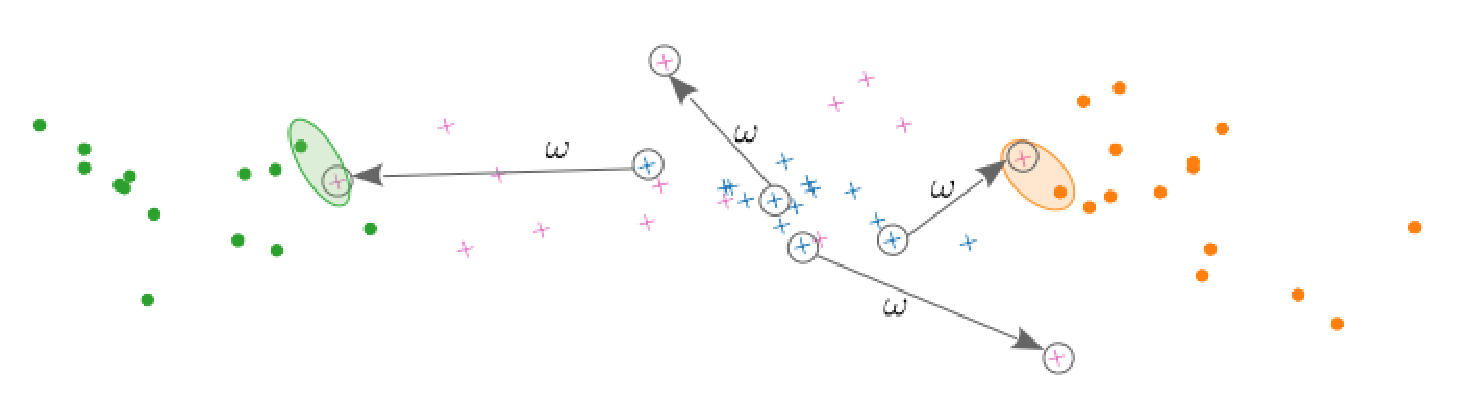
\includegraphics[width=0.75\linewidth]{ChapterThree/consistency.pdf}}
    \caption{Toy illustration of the desired effect of the consistency regularization, where images are represented as lying on a 2-D space. Green and orange circles represent (labeled) samples from two distinct source domains; blue and purple x-markers represent original and augmented (unlabeled) target samples, respectively. Colored ellipses enclose pairs of augmented and source samples that are close to each other and therefore are likely to share the same label.}
    \label{fig:consistency}
\end{figure}

The particular type of consistency regularization we adopt here is FixMatch (\citet{Sohn2020}), due to its simplicity and good performance. This approach involves using the predicted class of original (or weakly-transformed) samples as pseudo-labels for the (strongly-)transformed samples and, in our setting, is translated into the following loss function:
\begin{equation}
    L_{\text{cons}}(\vtheta_g, \vtheta_h) \triangleq -\frac{1}{m}\sum_{\vx \in \widehat{\gT}^{(m)}} \1_{\left(\max_{\ry \in \gY}\, p(\ry \mid \vx; \vtheta_g, \vtheta_h) > \tau \right)} \log p(\tilde{y} \mid \omega(\vx, \xi); \vtheta_g, \vtheta_h),
\end{equation}
where $\tilde{y} \triangleq \argmax_{\ry \in \gY} p(\ry \mid \vx; \vtheta_g, \vtheta_h)$ is the pseudo-label, $\xi$ is chosen randomly for each $\vx$, and $\tau \geq 0$ is a hyperparameter defining the minimum confidence threshold for the loss to be active. This threshold prevents the loss to be applied too early in the training process and, in our setting, may discard augmented samples that fall too far from the source distributions. The overall objective is then written as follows:
\begin{equation}
    \min_{\valpha \in \Delta, \vtheta_g, \vtheta_h}\max_{\vtheta_d} \Big\{ L \triangleq L_\text{class}(\valpha, \vtheta_g, \vtheta_h) + \mu_c \gL_\text{cons}(\vtheta_g, \vtheta_h) - \mu_d \gL_\text{disc}(\valpha, \vtheta_g, \vtheta_d) + \mu_s ||\valpha||_2^2 \Big\},
\end{equation}
where $\mu_c > 0$ controls the relative weight of the consistency loss. A full schematic of our model is provided in Appendix \ref{sec:model_overview}.\todo{Maybe add something about the causal interpretation of this heuristic}

It remains to discuss how to build the transformation $\omega$ in such a way that it is strong and diverse enough while satisfying the constraint of being label-preserving. This is essentially an application-dependent problem, though. For vision applications, there are multiple simple label-preserving transformations (e.g.\ translation, rotation, sharpness enhancement, etc.) that can be applied in a pipeline and, as consequence, the transformed image ends up being a strongly distorted version of the original one. This is the idea followed, for instance, in RandAugment (\citet{Cubuk2019}), which we use here. RandAugment receives as input parameters the magnitude and the number of transformations to be applied and randomly chooses the transformations to apply to each sample in the mini-batch. Here, as \citet{Sohn2020} did, we choose the number and magnitude of the transformations uniformly at random for each mini-batch.

For generic, non-vision problems, adding random noise sampled from some known distribution (e.g.\ Gaussian) is a trivial realization of $\omega$. Another possibility is to apply a strong dropout (\citet{Srivastava2014}) transformation at the input and inner layers of the neural network. Although such transformation is not necessarily label-preserving, dropout is known to be a successful regularization technique when applied at fully connected layers. We employ this idea in one of the experiments conducted here.

\subsection{Experiments}
\label{sec:modafm_experiments}

\subsubsection{Experimental protocol}
We now conduct several experiments using standard benchmark datasets for multi-source DA. We follow established evaluation protocols for every dataset and, as far as possible, we use the same network architecture for our model and baselines. Notably, comparing with MDAN (\citet{Zhao2018}), our single domain discriminator has the same architecture as each of the $k$ domain discriminators in their model. Consequently, our model has less trainable parameters than theirs. Our parameter $\vbeta$ is initialized uniformly at random in $[0,1]^k$, so the resulting $\valpha$ initially weights all source domains roughly equally, but it may become sparse as training evolves. We illustrate this behavior in Appendix \ref{sec:alpha_evol}. Hyperparameter tuning was performed through cross-validation over source domains and a hyperparameter sensitivity analysis is conducted in Appendix \ref{sec:hyperparam}. Further details about the experiments, including the label distributions on each domain (Appendix \ref{sec:label_dist}), network architectures (Appendix \ref{sec:arch}), search ranges for each hyperparameter (Appendix \ref{sec:cross_val}), and image transformations (Appendix \ref{sec:img_transf}), are also provided as appendices. The PyTorch-based implementation of our model is publicly available.\footnote{\url{https://github.com/dpernes/modafm}} To facilitate the presentation, from now on we refer to our model as MODA-FM (Multi-source mildly Optimistic Domain Adaptation with FixMatch regularization).

\paragraph{Baselines} DANN-SS (\citet{Ganin2015}): a single-source DA model, where the best results among all source domains are reported. DANN-MS: the same model as before trained on the combined data from all source domains. MADA (\citet{Pei2018})I: a state of the art model for single-source DA which tries to align conditional distributions by using one domain discriminator per class (results extracted from \citet{Pei2018}, we report the best accuracy among all source domains). MDAN (\citet{Zhao2018}): a model for multi-source DA, widely described before. MoE (\citet{Guo2018}): a state of the art model for multi-source DA that uses one classifier per source domain whose predictions are weighted in an example-dependent way. M$^3$SDA-$\beta$ (\citet{Peng2019}): a moment-matching model for multi-source DA in which two classifiers per source domain are trained to have maximum label discrepancy on the target domain (results extracted from \citet{Peng2019}). Fully supervised: fully supervised model trained on the target data, to provide an empirical upper bound on the performance of the DA task. MODA: our model without consistency regularization (i.e.\ $\mu_c = 0$). FM: our model without domain discriminator, trained on the naively combined data from all source domains and using FixMatch consistency regularization as described in \Secref{sec:modafm_consistency}.

\paragraph{Digits classification} In this experiment, the task is digit classification using 4 datasets: MNIST (\citet{LeCun1998}), MNIST-M (\citet{Ganin2015}), SVHN (\citet{Netzer2011}), and SynthDigits (\citet{Ganin2015}). We take each of the first three datasets as the target in turn, and use the remaining as source domains. The number of training images chosen randomly from each domain, including the target, is 20k. The evaluation is performed in the non-transductive setting, i.e. no target data used during training are used for evaluation. The results are in \Tableref{tab:digits_office_acc}.

\begin{table}
    \centering
    \resizebox{\linewidth}{!}{
    \begin{tabular}{l|ccc:c|ccc:c}
        \multicolumn{1}{c|}{} & \multicolumn{4}{c|}{Digits} & \multicolumn{4}{c}{Office-31} \\
        & MNIST                        & MNIST-M                       & SVHN  & Avg.                        & Amazon                        & DSLR                              & Webcam & Avg.                      \\ \hline
        DANN-SS \cite{Ganin2015}  & $ 97.9 $ \tiny{$ \pm 0.4 $}  & $ 73.2 $\tiny{$ \pm 1.6 $}   & $ 72.8 $ \tiny{$ \pm 3.3 $} & $81.3$ & $ 60.5 $ \tiny{$ \pm 1.4 $}   & $\boldsymbol{100.0}$ \tiny{$\pm 0.0$}     & $ 98.0$     \tiny{$ \pm 0.3 $} & $86.2$\\
        DANN-MS \cite{Ganin2015}  & $ 97.9 $ \tiny{$ \pm 1.6 $}  & $ 67.5 $ \tiny{$ \pm 1.4 $}   & $ 71.5 $ \tiny{$ \pm 1.6 $} & $79.0$ & $ 61.2 $ \tiny{$ \pm 1.3 $}   & $ 99.9 $ \tiny{$ \pm 0.2 $}       & $ 98.8 $ \tiny{$ \pm 0.3 $} & $86.6$\\
        MADA \cite{Pei2018}       & --                        & --                             & --                         & --  & $ 70.3 $ \tiny{$ \pm 0.3 $}   & $ 99.6 $ \tiny{$ \pm 0.1 $}       & $ 97.4 $ \tiny{$ \pm 0.1 $} &  $89.1$\\
        MDAN \cite{Zhao2018}      & $ 98.3 $ \tiny{$ \pm 0.2 $}  & $ 69.1 $ \tiny{$ \pm 1.2 $}   & $ 69.5 $ \tiny{$ \pm 2.8 $} & $79.0$ & $ 65.2 $ \tiny{$ \pm 0.4 $}   & $ 99.3 $ \tiny{$ \pm 0.2 $}       & $ 97.8 $ \tiny{$ \pm 0.5 $} & $87.4$\\
        MoE \cite{Guo2018}       & $ 98.6 $ \tiny{$ \pm 0.2 $}                     & $ 69.9 $ \tiny{$ \pm 1.1 $}                      & $ 81.8 $ \tiny{$ \pm 0.8 $}  & $83.4$ & --                            & --                                & --                          & --\\ \hline
        MODA         & $ 98.4 $ \tiny{$ \pm 0.2 $}  & $ 77.4 $ \tiny{$ \pm 1.6 $}   & $ 71.7 $ \tiny{$ \pm 1.5 $} & $82.5$ & $ 65.5 $ \tiny{$ \pm 0.5 $}   &   $ 99.9 $ \tiny{$ \pm 0.2 $}     & $ 99.0 $ \tiny{$ \pm 0.3 $}  & $88.1$\\
        FM           & $\boldsymbol{99.2}$ \tiny{$\pm 0.1$} & $ 91.1 $ \tiny{$ \pm 0.4 $}   & $\boldsymbol{90.0}$ \tiny{$\pm 0.8$} & $93.4$ & $ 70.3 $ \tiny{$ \pm 0.6 $}   & $ 99.7 $ \tiny{$ \pm 0.2 $}       & $\boldsymbol{99.2}$ \tiny{$\pm 0.4$} & $89.7$\\
        MODA-FM                      & $ 98.8 $ \tiny{$ \pm 0.1 $}  & $\boldsymbol{95.4}$ \tiny{$\pm 0.4$}  & $ 89.4 $ \tiny{$ \pm 1.4 $} & $\boldsymbol{94.5}$ & $\boldsymbol{70.7}$ \tiny{$\pm 0.9$}  & $ \boldsymbol{100.0} $ \tiny{$ \pm 0.0 $} & $ 99.1 $ \tiny{$ \pm 0.1 $} & $\boldsymbol{89.9}$\\ \hline
        Fully supervised            & $ 98.9 $ \tiny{$ \pm 0.1 $}  & $ 96.2 $ \tiny{$ \pm 0.1 $}   & $ 90.3 $ \tiny{$ \pm 0.5 $} & $95.1$ & $ 88.1 $ \tiny{$ \pm 1.6 $}   & $ 99.3 $ \tiny{$ \pm 1.1 $}       & $ 99.5 $ \tiny{$ \pm 0.7 $} & $95.6$
    \end{tabular}}
    \caption{Average accuracy $\pm$ standard deviation (\%) over 5 independent runs on digits and objects classification (Office-31). The domain on each column corresponds to the target.}
    \label{tab:digits_office_acc}
\end{table}

\paragraph{Object classification on Office-31 dataset} Office-31 (\citet{Saenko2010}) is a standard benchmark dataset for domain adaptation. It comprises 31 object categories extracted from 3 domains: Amazon, which contains 2817 images downloaded from \url{amazon.com}, DSLR and Webcam, which contain 498 and 795 images captured with DSLR cameras and webcams, respectively, under different environments. In this experiment, we adopt the fully-transductive setting, following \citet{Pei2018}, where all unlabeled data from the target domain are used for training (except for the fully supervised model, where we use 80\% of the data for training and the remaining for testing). All models are implemented using a pre-trained (on ImageNet) ResNet-50 (\citet{He2016}) as the base architecture. We take each domain as the target in turn and all remaining are used as sources. The results are presented in \Tableref{tab:digits_office_acc}.

\paragraph{Sentiment analysis on Amazon Reviews dataset} The Amazon Reviews dataset (\citet{Blitzer2007}) is another multi-domain dataset widely used as a benchmark for domain adaptation. It contains binary (i.e.\ positive and negative) reviews on four types of products: books, DVDs, electronics, and kitchen appliances. Here, we follow the experimental setting from \citet{Chen2012}, where samples were pre-processed to 5k-dimensional TF-IDF feature vectors, thus word order information was not preserved. We choose 2k training samples from each domain randomly and the remaining target samples are used for testing, following the non-transductive setting. Since the data are not images, we use dropout as our (pseudo-)label-preserving transformation. Specifically, on each training iteration, we randomly choose a dropout rate (in a pre-specified range) to be applied at the input and hidden layers of the multi-layer perceptron (MLP) and the corresponding output prediction is used as the pseudo-label $\tilde{y}$. No dropout is applied for source and non-augmented target samples. All domains are taken as the target in turn and all remaining are used as sources. The results are in~\Tableref{tab:amazon_acc}.

\begin{table}[]
    \centering
    \begin{tabular}{l|cccc:c}
        & Books           & DVD             & Electronics     & Kitchen  & Avg. \\ \hline
        DANN-SS \cite{Ganin2015} & $ 77.5 $ \tiny{$ \pm 1.0 $} & $ 78.9 $ \tiny{$ \pm 0.9 $} & $ 84.2 $ \tiny{$ \pm 0.2 $} & $ 85.8 $ \tiny{$ \pm 0.4 $} & $81.6$ \\
        DANN-MS \cite{Ganin2015} & $ 78.9 $ \tiny{$ \pm 0.2 $} & $ 80.8 $ \tiny{$ \pm 1.0 $} & $ 84.7 $ \tiny{$ \pm 0.6 $} & $ 87.0 $ \tiny{$ \pm 0.4 $} & $82.9$ \\
        MDAN \cite{Zhao2018}     & $ 79.1 $ \tiny{$ \pm 0.3 $} & $ 81.3 $ \tiny{$ \pm 0.8 $} & $ 84.6 $ \tiny{$ \pm 0.3 $} & $ 85.6 $ \tiny{$ \pm 1.6 $} & $82.7$ \\
        MoE \cite{Guo2018}      & $ 80.3 $ \tiny{$ \pm 0.3 $} & $ 81.9 $ \tiny{$ \pm 0.6 $} & $ 85.2 $ \tiny{$ \pm 0.6 $} & $ 87.4 $ \tiny{$ \pm 0.5 $} & $83.7$\\ \hline
        MODA     & $ 79.0 $ \tiny{$ \pm 0.2 $} & $ 80.7 $ \tiny{$ \pm 1.2 $} & $ 84.7 $ \tiny{$ \pm 0.3 $} & $ 86.8 $ \tiny{$ \pm 0.6 $} & $82.8$\\
        FM         & $ 78.8 $ \tiny{$ \pm 2.0 $} & $ 81.0 $ \tiny{$ \pm 1.5 $} & $\boldsymbol{85.6}$ \tiny{$\pm 0.9 $} & $ 87.6 $ \tiny{$ \pm 0.7 $} & $83.3$\\
        MODA-FM    & $\boldsymbol{80.9}$ \tiny{$\pm 1.1$} & $\boldsymbol{82.0}$ \tiny{$\pm 1.0$} & $ 85.3 $ \tiny{$ \pm 0.4 $} & $\boldsymbol{88.4}$ \tiny{$\pm 0.3$} & $\boldsymbol{84.2}$\\ \hline
        Fully supervised & $ 83.6 $ \tiny{$ \pm 0.4 $} & $ 83.6 $ \tiny{$ \pm 0.6 $} & $ 85.4 $ \tiny{$ \pm 0.4 $} & $ 87.8 $ \tiny{$ \pm 0.2 $} & $85.1$
    \end{tabular}
    \caption{Average accuracy $\pm$ standard deviation (\%) over 5 independent runs on sentiment analysis (Amazon Reviews). The domain on each column corresponds to the target.}
    \label{tab:amazon_acc}
\end{table}

\paragraph{Large scale object classification on DomainNet dataset} To the best of our knowledge, the DomainNet dataset (\citet{Peng2019}) is the largest domain adaptation image dataset to date. It consists of 6 domains, each containing 345 categories of common objects. The domains are: clipart images (\textit{clp}), infographic images (\textit{inf}), artist paintings (\textit{pnt}), drawings made by worldwide players of the game ``Quick, Draw!" (\textit{qdr}), real world images (\textit{rel}), and sketches of objects (\textit{skt}). The dataset consists of around 423.5k images split in prespecified train/test partitions. For training the models, we use all the data from the training partition, excluding the labels for the target domain. For testing, we use the target domain data from the test partition. All models were implemented on top of a pre-trained (on ImageNet) ResNet-152. All domains are taken as the target in turn and all remaining are used as sources. The results are in~\Tableref{tab:domainnet_acc}.

\begin{table}[]
    \centering
    \begin{tabular}{l|cccccc:c}
        & \textit{clp} & \textit{inf} & \textit{pnt} & \textit{qdr}  & \textit{rel} & \textit{skt} & Avg. \\ \hline
        DANN-MS \cite{Ganin2015} & $\boldsymbol{62.6}$ & $21.7$  & $50.3$ & $14.3$ & $\boldsymbol{63.5}$ & $48.3$ & $43.5$ \\
        MDAN \cite{Zhao2018} & $52.2$ & $19.1$ & $46.0$ & $12.6$ & $48.2$& $40.4$ & $36.4$\\
        M$^3$SDA-$\beta$ \cite{Peng2019} & $58.6$& $\boldsymbol{26.0}$& $\boldsymbol{52.3}$ & $6.3$& $62.7$ & $49.5$ & $42.6$\\ \hline
        MODA-FM       & $61.2$ & $24.5$  & $51.2$  & $\boldsymbol{17.2}$  & $62.3$ & $\boldsymbol{52.4}$ & $\boldsymbol{44.8}$\\ \hline
        Fully supervised & $68.5$ & $28.7$ & $61.5$ & $64.5$ & $78.5$ & $59.3$ & $60.2$
    \end{tabular}
    \caption{Accuracy on object classification (DomainNet). The domain on each column corresponds to the target.}
    \label{tab:domainnet_acc}
\end{table}

\subsubsection{Discussion}
Tables \ref{tab:digits_office_acc}, \ref{tab:amazon_acc}, and \ref{tab:domainnet_acc} show that our model outperforms the baselines in most settings and performs comparably to the fully-supervised model in many. When no consistency regularization is used (MODA), our approach exhibits a higher accuracy than DANN-SS, DANN-MS and MDAN in most cases. This observation shows that our mildly optimistic combination of source domains works better than using only the data from the best source domain (DANN-SS) or naively combining the data from all source domains (DANN-MS). It also suggests that MDAN wastes too much computational effort on optimizing itself for the hardest source domain. MADA and MoE perform better than our non-regularized model in some cases, which is not surprising since both methods try to mitigate somehow the curse of domain-invariant representations. Their advantage is, therefore, mostly noticeable when the target shift is large (e.g.\ SVHN and all domains in Office-31 -- see Appendix \ref{sec:label_dist}), but the performance is still below MODA-FM.

Very significant performance gains are observed when we apply the consistency regularization, particularly in the visual datasets (digits and Office-31). These gains are more expressive in the most challenging settings, i.e.\ when the target data are perceptually very different from the source data (e.g.\ MNIST-M -- see Appendix \ref{sec:sample_imgs}) or when the target shift is large. The latter observation suggests that this regularization succeeds on mitigating the curse of domain-invariant representations, as hypothesized before. This is strongly corroborated by an experiment we present in Appendix \ref{sec:overtrain}, where we show that the model accuracy on the target domain keeps stably high when the model is trained for a large number of epochs. Interestingly, though, we observe that, in some settings, FM outperforms MODA-FM, although the differences are small. In these cases domain-invariant representations are slightly hurting the performance and/or the source weights $\alpha$ are sub-optimal. Besides being the largest dataset, DomainNet is also the most challenging for the DA task. For almost all domains, there is a large gap between the performance of all DA models (including ours) and the fully supervised. Interestingly, none of the multi-source DA algorithms does much better than the naive DANN-MS for this particular dataset. This might be explained by the large dissimilarity across domains in DomainNet: since no source domain is particularly close to the target domain, weighting all source domains equally works ends up working fairly well. Nonetheless, our model achieves the best average performance across all source domains.  Finally, it is worth highlighting the positive effect provided by using dropout as the label-preserving transformation $\omega$ in the experiment with Amazon Reviews. This observation suggests that this methodology can be applied successfully to non-visual data too.

\subsection{Conclusion}
\label{sec:modafm_conclusion}
We have presented a novel algorithm that achieves state of the art results in unsupervised multi-source domain adaptation. In our approach, the problem is formulated as DA from a single source domain whose distribution corresponds to a mixture of the original source domains. The mixture weights are adjusted dynamically throughout the training process, according to a mildly optimistic objective. Additionally, we employ FixMatch on the target samples, a form of consistency regularization that proves to have a strong impact on the model performance and to be capable of mitigating the curse of domain-invariant representations. This regularization relies on a label-preserving transformation, which is hard to construct for non-visual data. Moreover, better results could be achieved if both the label-preserving transformation and the source weights were learned to approximate the augmented target samples to the source samples. Both problems are interesting lines for future research.

\section{Summary}
\label{sec:da_summary}
In this chapter, we addressed the problem of domain adaptation, a particular type of transfer learning where the label space $\gY$ is constant across domains (i.e.\ the learning task is the same on source and target domains). Contrary to Chapter \ref{chp:networked_data_streams}, where the goal was to exploit correlations in data from multiple entities to build a model with good performance across all training domains, in DA the focus is on a specific entity/domain for which no labeled data is available.

In \Secref{sec:da_sensors}, we investigated several strategies to combine a multi-source DA algorithm with a CNN for object counting in videos. The purpose was to build a robust model capable of generalizing well to new cameras with different points of view, without the need to collect further annotated data. Moreover, this was one of the first few attempts to extend the success of adversarial DA techniques to temporal data and, in particular, to video sequences, a topic that has been seldom explored in the literature.

In \Secref{sec:modafm}, we presented our novel algorithm for unsupervised multi-source DA, the main contribution of this chapter. This algorithm builds upon existing methods by i) learning to weight source domains jointly with the minimization of source error and alignment of marginal distributions and ii) employing a regularization technique that proved to successfully mitigate the curse of domain-invariant representations, particularly for image data. The latter had a highly beneficial effect on the performance and was therefore crucial for the state of the art results achieved by this model.